 \hoffset1cm % przesunięcie poziome (przykładowo) o 1cm przeznaczone na oprawę

 \documentclass[11pt]{report}
 
 \usepackage[T1]{fontenc}
 \usepackage[utf8]{inputenc}
 \usepackage{graphicx}
 \usepackage{amsmath,amssymb,amsfonts}
 \usepackage{polski}
 \usepackage[raggedright]{titlesec}
 \usepackage{amsmath}
 \usepackage{amssymb}
 \usepackage{indentfirst}
 \usepackage{listings}
 \usepackage{hyperref}
 \usepackage[backend=biber, bibencoding=utf8, style=ieee, isbn=false, doi=false, sorting=anyvt]{biblatex}
 
 \addbibresource{library.bib}
 \DeclareUnicodeCharacter{229}{ę}
 \DeclareUnicodeCharacter{327}{}
 
 \pagestyle{headings}
 
 \renewcommand{\chaptername}{Rozdział}
 \renewcommand{\contentsname}{Spis treści}
 \renewcommand{\figurename}{Rys.}
 \renewcommand{\tablename}{Tab.}
 \renewcommand{\listfigurename}{Spis rysunków}
 \renewcommand{\listtablename}{Spis tabel}
 \renewcommand{\bibname}{Bibliografia}

\makeatletter
\renewcommand{\l@section}{\@dottedtocline{1}{1.5em}{2.6em}}
\renewcommand{\l@subsection}{\@dottedtocline{2}{4.0em}{3.6em}}
\renewcommand{\l@subsubsection}{\@dottedtocline{3}{7.4em}{4.5em}}
\makeatother


 \begin{document}

 \begin{titlepage}
 \center{\large\scshape Politechnika Krakowska \\
         \normalsize im. Tadeusza Kościuszki}
 \center{\scshape Wydział Inżynierii Elektrycznej i Komputerowej\\
         Kierunek Informatyka}
 \vspace{0.1\textheight}
 \center{\scshape Michał Patyk}
 \bigskip
 \center{\LARGE\bfseries Sterownik pieca kominkowego, w oparciu o mikrokontroler (lub platformę komputerową), zgodny ze szkicem specyfikacji Web Thing API}
 \center{(praca inżynierska)}
 \vspace{0.3\textheight}
 \par
 \rightline{Promotor: dr inż. Radosław Czarnecki}

 \vspace{0.1\textheight}
 \center{Kraków 2020}
 \end{titlepage}


 \tableofcontents


 \chapter{Wstęp}
 
 \section{Rys historyczny - ujęcie problemowe}
 \subsection{Problem ogrzewania}
 Problem ogrzewania pomieszczeń towarzyszy człowiekowi od zarania dziejów \cite{Hoppe2018}. Zwykle był to proces wymagający ciągłego nadzoru. Potrzeba automatyzacji wydaje się naturalną konsekwencją zmiany trybu życia człowieka. Wraz z pojawieniem się nowoczesnych kotłów, powstały pierwsze mechanizmy kontrolujące pracę urządzenia bez nieustannej konieczności doglądania go.
 Pojawienie się sterowników cyfrowych zaoferowało zupełnie nowe możliwości, takie jak:
  \begin{enumerate}
 \item[•] większą efektywność pracy systemu grzewczego
 \item[•] zmniejszenie emitowanych zanieczyszczeń
 \item[•] wzrost komfortu użytkowania
 \item[•] poprawę bezpieczeństwa
 \item[•] zdalne sterowanie (w nowszych modelach)
  \end{enumerate}
 Sterowniki cyfrowe wydają się również odpowiedzią na coraz bardziej dostrzegany problem odpowiedzialnego wykorzystywania zasobów naturalnych \cite{Mazurek2018}\cite{Mazurek2018a}, gdyż za ich pomocą do zapewnienia komfortu termicznego pomieszczeń potrzebna jest znacznie mniejsza ilość paliwa. Stanowią one również propozycję rozwiązania problemu ubóstwa energetycznego.
 \subsection{Integracja urządzeń}
 Sukces internetu spowodował zainteresowanie naukowców podłączeniem do sieci fizycznych urządzeń.
 Termin internet rzeczy powstał w 1999 roku wymyślony przez Kevina Ashtona \cite{Ashton2009} jednak jego popularność rozpoczęła się dopiero kilka lat temu, a w tej chwili przechodzi okres stagnacji.
 Możemy wyróżnić wiele przypadków zastosowania internetu rzeczy:
 \begin{enumerate}
 \item[•] bezprzewodowe sieci czujników i pomiary rozproszone,
 \item[•] urządzenia ubieralne i urządzenia do pomiaru parametrów zdrowia,
 \item[•] inteligentne domy i budynki,
 \item[•] inteligentne miasta i sieci energetyczne,
 \item[•] inteligentna produkcja przemysłowa,
 \item[•] inteligentna logistyka i łańcuchy dostaw.
\end{enumerate}
 Przyjęte przez niewielkie grupy korporacji standardy internetu rzeczy podlegają ciągłej ewolucji spowodowanej rozwojem technologicznym, a zamknięte protokoły prowadzą do sytuacji, w której zmiana dostawcy rozwiązań jest mocno utrudniona i może powodować konieczność zmiany sprzętu. Standardy webowe, takie jak HTTP, JSON i Web Socket, zawdzięczają swoją popularność otwartości oraz brakowi opłat. Ich zastosowanie do integracji urządzeń i aplikacji w znacznym stopniu może ułatwić wchodzenie w interakcję z rzeczami.
 
 \section{Stan aktualnej wiedzy}
 \subsection{Sterowniki}
 Obecnie na rynku dostępny jest szeroki wachlarz rozwiązań, od prostych jednokomponentowych do bardziej zaawansowanych i złożonych. Począwszy od regulatorów pokojowych, które jedynie włączają ogrzewanie kiedy temperatura pomieszczenia obniży się poniżej nastawionej wartości, poprzez rozbudowane, umożliwiające programowanie temperatury zarówno w ciągu doby (niższa w nocy, wyższa po południu), jak i w wybrane dni tygodnia. Skończywszy na automatyce pogodowej, która dzięki wykorzystaniu czujnika zewnętrznego, umieszczonego na ścianie domu, przewiduje zwiększone zapotrzebowanie na ciepło i wcześniej dostosowuje moc kotła.
 Coraz więcej dostępnych na rynku sterowników umożliwia zdalne nastawienie temperatury. W znakomitej większości standard komunikacji tych rozwiązań jest zamknięty, co utrudnia współpracę  z innymi inteligentnymi urządzeniami.
 \subsection{Internet rzeczy i WWW rzeczy}
 W Europie Wschodniej występuje wciąż mała na tle konkurencji liczba firm oferujących rozwiązania IoT.
  \begin{figure}[ht]
\centering
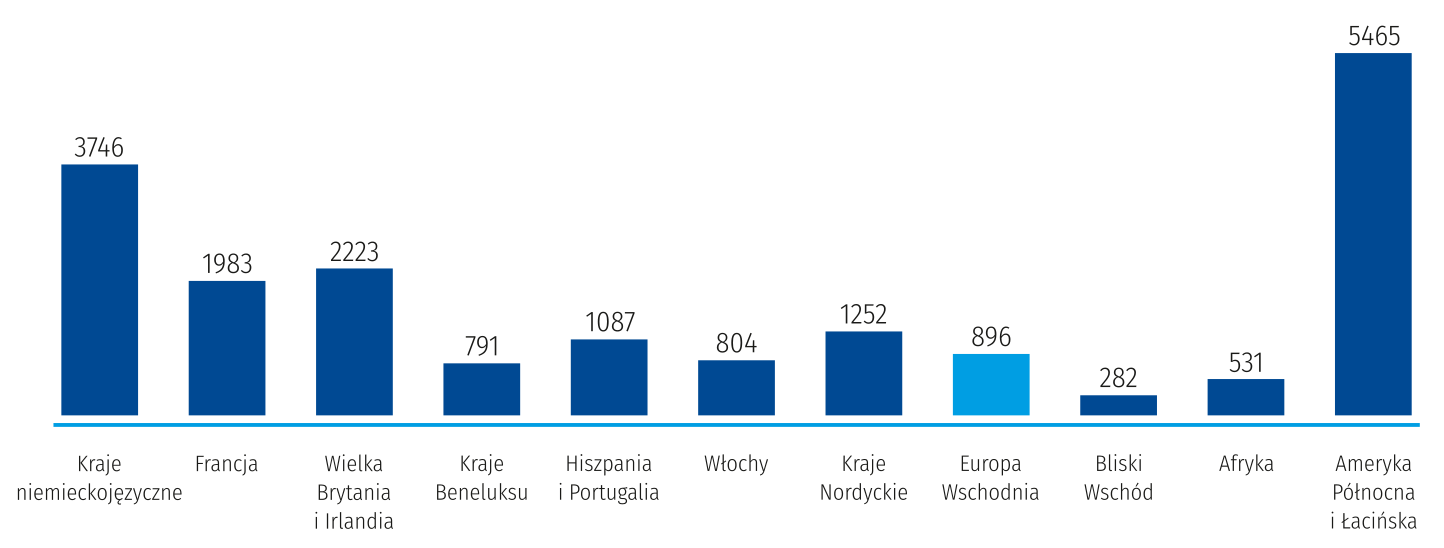
\includegraphics[width=0.8 \textwidth]{fig/liczba_firm_rozwiazania_iot.png}
\caption{Liczba firm oferujących rozwiązania IoT na poszczególnych rynkach. (źródło: \cite{gov2019})}
\label{fig:firmy}
\end{figure}
 Wzmożony rozwój tematu WWW rzeczy zapoczątkowany został przez pracę doktorską Dominique'a Guinarda \cite{Guinard2011}, a pogłębiło go wydanie książki \cite{Guinard2017} podsumowującej dotychczasowe prace autora w tym temacie \cite{Guinard2009} \cite{Guinard2010} \cite{Guinard2010a} \cite{Guinard2011} \cite{Guinard2011a}.
 W 2014 roku przy World Wide Web Consortium, grupie zajmującej się ustanawianiem standardów pisania i przesyłu stron WWW, powstała Web of Things Interest Group \cite{wotig2014} która pracuje nad dokumentami opisującymi Rzeczy Webowe \cite{thingdescription} oraz Architekturę \cite{wotarchitecture}.
 W 2017 roku do projektowania Web of Things przyłącza się fundacja Mozilli \cite{mozilla2017} tworząc i rozbudowując projekt WebThings Gateway. Przyciągnął on liczną i aktywną społeczność znacząco rozwijającą przedsięwzięcie.  W następnych latach przybywa kolejnych prac naukowych na temat Web of Things \cite{IEEE2018} \cite{Raggett2018} \cite{Korkan2019}.
   \begin{figure}[ht]
\centering
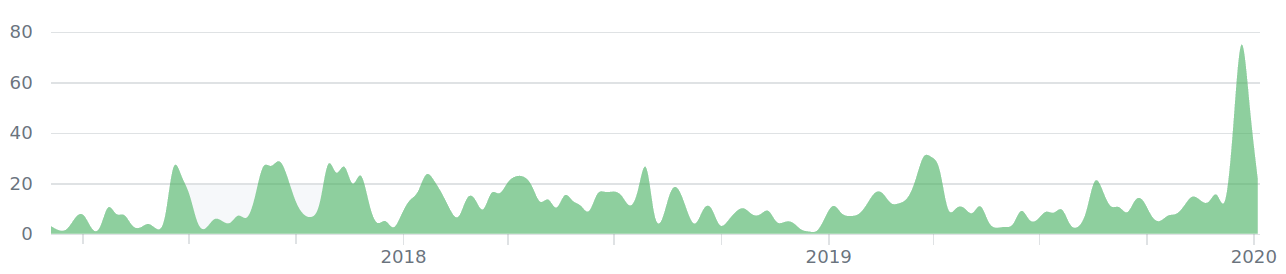
\includegraphics[width=0.8 \textwidth]{fig/contributions.png}
\caption{Liczba przesłanych fragmentów kodu przez społecznośc WebThings Gateway. (zródło: \cite{gatewaycommits2020})}
\label{fig:contributions}
\end{figure}

 \section{Innowacyjność projektu na tle współczesnych rozwiązań}
 W odróżnieniu od szeroko stosowanych rozwiązań projekt zakłada użycie specyfikacji Web Thing API \cite{WebThing2020}, która pozwala na ujednolicenie dostępu do inteligentnych rzeczy za pomocą dodatkowej warstwy abstrakcji. Oznacza to, że system kreuje przestrzeń kooperacji urządzeń. Możliwe interakcje wpływają pozytywnie na koherentność systemu.
 
 \section{Motywacja}
Pomysł na pracę zrodził się z potrzeby zmniejszenia ilości czasu oraz poświęcanej uwagi potrzebnych do obsługi pieca kominkowego, pracującego jako główne źródło ciepła w domu jednorodzinnym. Ponadto niekomfortowym ograniczeniem dotychczas stosowanych rozwiązań jest zmuszanie klienta do użytkowania produktów pochodzących od tego samego producenta, co w znaczącym stopniu ogranicza możliwość wyboru preferowanego sprzętu.


 \chapter{Cele pracy, zakres pracy, założenia}\label{ch:cele}

 \section{Cele pracy}
 Celem niniejszej pracy jest \textbf{opracowanie koncepcji sterownika pieca kominkowego} zgodnego ze szkicem specyfikacji Web Thing API oraz \textbf{stworzenie dedykowanego oprogramowania}.

 \section{Zakres pracy}
 Zakres pracy obejmuje:
 \begin{enumerate}
 \item przegląd istniejących rozwiązań - zarówno sprzętowych jak i programowych;
 \item opracowanie koncepcji;
 \item wybór podzespołów;
 \item wykonanie prototypu na płytce stykowej;
 \item stworzenie oprogramowania;
 \item przetestowanie oprogramowania; 
 \item wykonanie prototypu na płytce uniwersalnej;
 \item wykonanie obudowy;
 \item zintegrowanie z Mozilla Gateway
 \end{enumerate}
 
 \section{Założenia i wymagania}
 Projekt sterownika zostanie wykonany zgodnie z dobrymi praktykami dotyczącymi programowania zawartymi między innymi w pracach Grębosza \cite{Grebosz2018} i Francuza \cite{Francuz2015}. Część sprzętowa projektu zostanie opracowana na podstawie książek Monka \cite{Monk2014} \cite{Monk2014a} \cite{Monk2018}, Kurczyka \cite{Kurczyk2019}, Huanga \cite{Huang2018} i Wallace'a \cite{Wallace2019} oraz norm Polskiego Komitetu Normalizacyjnego \cite{PKN1999} \cite{PKN2000}.
 
 \subsection{Wykorzystane narzędzia}
 \begin{enumerate}
 \item[•] środowisko programistyczne CLion
 \item[•] język programowania C/C++
 \item[•] ekosystem PlatformIO
 \item[•] platforma monitoringu i kontroli urządzeń WebThing Mozilla
 \end{enumerate}
 
 \subsection{Możliwości}
 \begin{enumerate}
 \item[•] monitorowanie pracy pieca kominkowego
 \item[•] zdalne zadawanie temperatur
 \item[•] informowanie o zdarzeniach
 \end{enumerate}
 
 \subsection{Wymagania}
 \begin{enumerate}
 \item[•] zgodność z Web Thing API
 \item[•] możliwość rozbudowy o dodatkowe czujniki i elementy wykonawcze
 \item[•] przywracanie nastaw po utracie zasilania
 \item[•] minimalizacja otwarcia przepustnicy w przypadku zaniku napięcia
 \item[•] sygnalizacja uszkodzenia czujnika temperatury
 \item[•] regulowana jasność wyświetlacza - zwiększana na czas zmiany ustawień
 \item[•] sygnalizator dźwiękowy który informuje gdy temperatura wzrośnie do niebezpiecznego poziomu
 \end{enumerate}
 
 \section{Efekt końcowy}
 Planowanym efektem końcowym pracy będzie stworzenie sterownika pieca kominkowego, pozwalającego na bezobsługową pracę paleniska pomiędzy momentami uzupełniania paliwa.

 Element wyróżniający wykonany sterownik stanowi wykorzystanie Web Thing REST API, który pozwala na wykorzystanie sieci, jako zunifikowanej warstwy abstrakcji, dla zdecentralizowanego internetu rzeczy.
 
 Rysunek~\ref{fig:wizja} przedstawia wizję struktury elementów sterownika.
 \begin{figure}[ht]
\centering
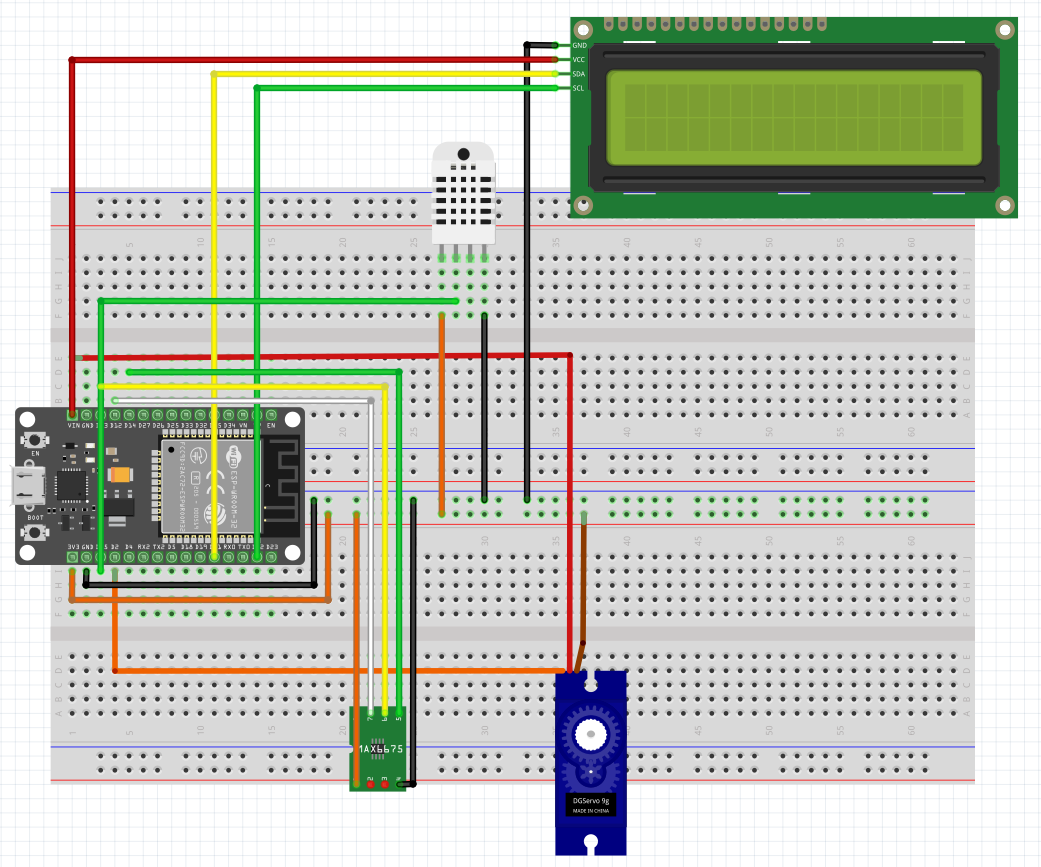
\includegraphics[width=0.8 \textwidth]{fig/fritzing_bredboard_v1.png}
\caption{Wizja elementów sterownika. (opracowanie własne)}
\label{fig:wizja}
\end{figure}
 
 \section{Dalsze kierunki rozwoju}
 W tej części zostaną opisane możliwe kierunki rozwoju sterownika.
 \subsection{Integracja z innymi urządzeniami}
 Wykorzystanie WebThing API umożliwi w przyszłości łatwą integrację sterownika z dodatkowymi urządzeniami, takimi jak:
 \begin{enumerate}
 \item[•] czujnik pogodowy
 \item[•] systemem odzyskiwania ciepła ze spalin
 \item[•] inne źródła ciepła
 \end{enumerate}
 \subsection{Zmiany w oprogramowaniu sterownika}
 Oprogramowanie sterownika może zostać rozbudowane o przykładowe komponenty:
 \begin{enumerate}
 \item[•] dodatkowe opcje konfiguracyjne
 \item[•] programowanie czasowe
 \item[•] zabezpieczenie hasłem
 \item[•] dodatkowe tryby pracy pieca
 \end{enumerate}
 Możliwą do wprowadzenia zmianą może być też zastąpienie frameworka Arduino, bardziej profesjonalnym Espressif IoT Development Framework, który lepiej współpracuje z mikrokontrolerem ESP32.
 \subsection{Zmiany sprzętowe}
 Proponowanymi zmianami w obrębie sprzętowym są:
 \begin{enumerate}
 \item[•] zaprojektowanie i wykonanie płytki drukowanej
 \item[•] zaprojektowanie i wykonanie dedykowanej obudowy, np.: w technologi druku 3D
 \end{enumerate}
 

 \chapter{Charakterystyka metod obsługi pieca}\label{ch:charakterystyka}
 Obsługa w pełni manualna wymaga stałego nadzoru nad przebiegiem spalania. Jest to bardzo absorbujące i często nieekonomiczne ze względu na łatwość przekroczenia pożądanych temperatur. Obsługa manualna pogarsza również efektywność procesu spalania, co prowadzi do obniżenia ogólnej sprawności kotła, większego zapotrzebowania na opał, a w konsekwencji znacznie wyższych kosztów ogrzewania.
 
 Obsługa półautomatyczna pozwala na samodzielną pracę urządzenia pomiędzy momentami dokładania paliwa. Można wyróżnić dwie jej odsłony:
 \begin{enumerate}
 \item[•] mechaniczna, w której głowica termostatyczna połączona jest z mechanizmem dźwigni. Na jej ramieniu znajduje się łańcuszek lub linka. Zaletą jest niski koszt;
 \item[•] elektroniczna, gdzie stosuje się sterownik pokojowy z serwomechanizmem. Koszt tego rozwiązania jest umiarkowany oraz zapewnia szerokie możliwości regulacji, umożliwiając dokonywanie nastaw lokalnie lub zdalnie. 
\end{enumerate}
 
 Najdroższe jak i najbardziej autonomiczne rozwiązanie stanowi obsługa automatyczna, w której kocioł z podajnikiem paliwa pracuje samodzielnie do kilku dni.
 
 
 \chapter{Przegląd istniejących rozwiązań}\label{ch:przeglad}
 \section{Standardy integracji inteligentnych urządzeń}
 W przypadku internetu rzeczy producenci nie zwracali uwagi na stworzenie otwartych systemów komunikujących się ze sobą urządzeń. Szczególnie ograniczone były działania  podejmowane dla umożliwienia doraźnego współdziałania elementów składających się na internet rzeczy. Pomimo, że organizacje standaryzacyjne zaproponowały wiele protokołów, żaden z tych standardów nie zdobył na tyle dużej popularności by zdominować pozostałe rozwiązania. Coraz więcej urządzeń podłączanych do internetu udostępnia API, jednak każdy z nich został zaimplementowany z wykorzystaniem innych protokołów i używa innego modelu danych. Zamiast proponować kompletnie nowe normy komunikacyjne, Web of Things wykorzystuje istniejące, dobrze znane standardy webowe.
  
 \section{Sterowniki kominkowe}
 Na polskim rynku istnieje szeroka gama rozwiązań przeznaczonych dla kotłów na paliwo stałe, jednak stosunkowo niewielką ilość sterowników przeznaczono dla kominków. Istnieją wyłącznie modele z dodatkową przepustnicą, co ogranicza możliwość regulacji dopływu powietrza pierwotnego i wtórnego.
 \subsection{TECH STEROWNIKI}
 Firma TECH ma w swojej aktualnej ofercie \cite{Tech} trzy sterowniki do kominków. Dwa z nich są do kominków z płaszczem wodnym. Trzeci \cite{TechSterownik} przeznaczony jest do kominków z dystrybucją gorącego powietrza i mógłby zostać zastosowany przy piecu kominkowym. Czujnik mierzy temperaturę spalin w kominie.
 Aby mieć możliwość zdalnego dostępu do sterownika należy skorzystać z jednego z dwóch dodatkowych modułów komunikacyjnych - GSM lub Ethernet. Dostęp jest możliwy jedynie przez stronę producenta lub aplikację mobilną, brak publicznego API.
 Sam moduł Ethernet kosztuje około 500zł \cite{TechEthernetCena}.
 \subsection{EUROSTER}
 Firma EUROSTER ma w swojej aktualnej ofercie \cite{Euroster} tylko jeden sterownik do kominków. Jest on \cite{EurosterSterownik} przeznaczony do współpracy z kominkiem z płaszczem wodnym, więc nie może być zastosowany do pieca kominkowego, gdyż czujnik mierzy temperaturę wody obiegowej, która nie występuje w piecu kominkowym. Sterownik nie posiada możliwości zdalnego dostępu.
 Cena samego sterownika to około 300zł \cite{EurosterSterownikCena}. Dodatkowo należy zakupić przepustnicę.
 \subsection{Kratki}
 Firma Kratki ma w swoje ofercie \cite{Kratki} jeden sterownik do kominków występujący w kilku wersjach różniących się obudową i wielkością dołączonej do zestawu przepustnicy.
 Jest on przeznaczony do współpracy z kominkami każdego rodzaju, dlatego może zostać zastosowany do pieca kominkowego. Czujnik mierzy temperaturę w pobliżu paleniska. Sterownik nie posiada możliwości zdalnego dostępu. 
 Cena samego sterownika to około 400zł \cite{KratkiSterownik}.
  \subsection{Podsumowanie}
  Tylko jeden z wymienionych producentów pozwala na zdalny dostęp do sterownika, jednak jest on wyłącznie możliwy za pośrednictwem serwerów producenta. Brak publicznego API. Koszt tego rozwiązania jest wysoki.
  Tylko jeden z wymienionych sterowników posiada czujnik pozwalający na mierzenie temperatury spalin.
  
  
 \chapter[Opracowanie koncepcji budowy sterownika\\ pieca kominkowego]{Opracowanie koncepcji budowy sterownika pieca kominkowego}\label{ch:koncepcja}
 Projektowanie koncepcji sterownika pieca kominkowego należy rozpocząć od skompletowania minimalnej wersji, na którą składa się: mikrokontroler, serwomechanizm oraz termopara. Do regulacji pracy pieca kominkowego jest potrzebne urządzenie potrafiące zmieniać położenie przepustnicy dolotu powietrza do komory spalania. Najbardziej optymalnym wyborem okazał się prosty serwomechanizm, którego dodatkową zaletą jest przystępna cena. Stopień otwarcia przepustnicy dobierany jest na podstawie temperatury spalin w kominie, mierzonej przez termoparę.
 Dodatkowymi elementami uzupełniającymi koncepcję są:
 \begin{enumerate}
 \item[•] termometr, mierzący temperaturę w pomieszczeniu, umożliwiający dobór mocy pieca w stosunku do zapotrzebowania na ciepło
 \item[•] wyświetlacz przekazujący informacje użytkownikowi
 \item[•] czujnik otwarcia drzwi paleniska umożliwiający zmianę parametry pracy po dołożeniu drewna
 \item[•] zdalny dostęp do sterownika w celu ułatwienia obsługi
 \item[•] moduł Ethernet pozwalający na usunięcie niepotrzebnego ruchu WiFi
 \item[•] zapasowe źródło zasilania, pozwalające na kontrolę pracy pieca w razie zaniku napięcia w sieci
 \item[•] przyciski na sterowniku do zmiany podstawowych parametrów
 \end{enumerate}  
 
  
 \chapter{Wybór podzespołów sterownika pieca kominkowego}\label{ch:wybor}
 \chaptermark{Wybór podzespołów sterownika...}
 \section{Mikrokontroler lub platforma komputerowa}
 Jako serce sterownika można wykorzystać:
 \begin{enumerate}
 \item platformy komputerowe:
 \begin{enumerate}
 \item[•] RaspberryPi
 \item[•] OrangePi
 \end{enumerate}
\item mikrokontrolery:
 \begin{enumerate}
 \item[•] Seria Arduino
 \item[•] STM32F103C8T6
 \item[•] ESP8266
 \item[•] ESP32
 \end{enumerate}
 \end{enumerate}
 Ze względu na koszt jak i rozdzielenie odpowiedzialności w pracy wybrano mikrokontrolera ESP32. Jest to układ System on Chip będący następcą ESP8266. Posiada on dwa rdzenie, moduł komunikacji WiFi oraz bluetooth. Wyróżnia go energooszczędność. Dużą zaletą jest stosunkowo niska cena (w Chinach około 25zł). Gotowa płytka deweloperska pozwala na wygodne prototypownie.
 
 \section{Wyświetlacz}
 Aby sterownik sprostał potrzebom użytkowników o pogorszonym wzroku, wyświetlacz powinien być duży i kontrastowy.
 Ze względu na to, że wszystkie parametry będą dostępne przez stronę internetową, wybrany został wyświetlacz LCD 2x16, który pozwoli na prezentowanie tylko kilku z nich w jednej chwili.
 
 \section{Termometr}
 Wybrany układ termometru DHT22 pozwala na pomiar temperatury i~wilgotności, jednocześnie zapewniając dobrą precyzję odczytów. Dodatkowo, sterownik rozszerzony został o moduł termometru Dallas DS18B20, który pozwala na pomiar temperatury wewnątrz urządzenia.
 
 \section{Termopara}
 W pracy wybrano układ MAX6675, który jest jednym z najlepiej przetestowanych i najtańszych rozwiązań, ze względu na swoją długą obecność na rynku.
 
 \section{Układ poruszający przepustnicą} 
 Posiadany piec kominkowy, który jest wzorcowy dla sterownika, potrzebuje przemieszczania liniowego przepustnicy, jednak odpowiednie serwomechanizmy są wciąż drogie i przewyższałyby swoją ceną koszt pozostałych podzespołów całego sterownika.
 Istnieje możliwość zaprojektowania i wydrukowania właściwego adaptera serwomechanizmu, lecz długi czas produkcji oraz testowania jego wytrzymałości przekraczałby zakres tej pracy.
  Ze względu na niewielką wymaganą precyzję ustawienia przepustnicy oraz zaistniałe opory, wybrano standardowej wielkości, analogowy serwomechanizm MG-995, bez adapterów przekształcających ruch obrotowy na liniowy.
   Zdjęcie~\ref{fig:servo} przedstawia serwomechanizm zainstalowany przy piecu kominkowym.
    \begin{figure}[ht]
\centering
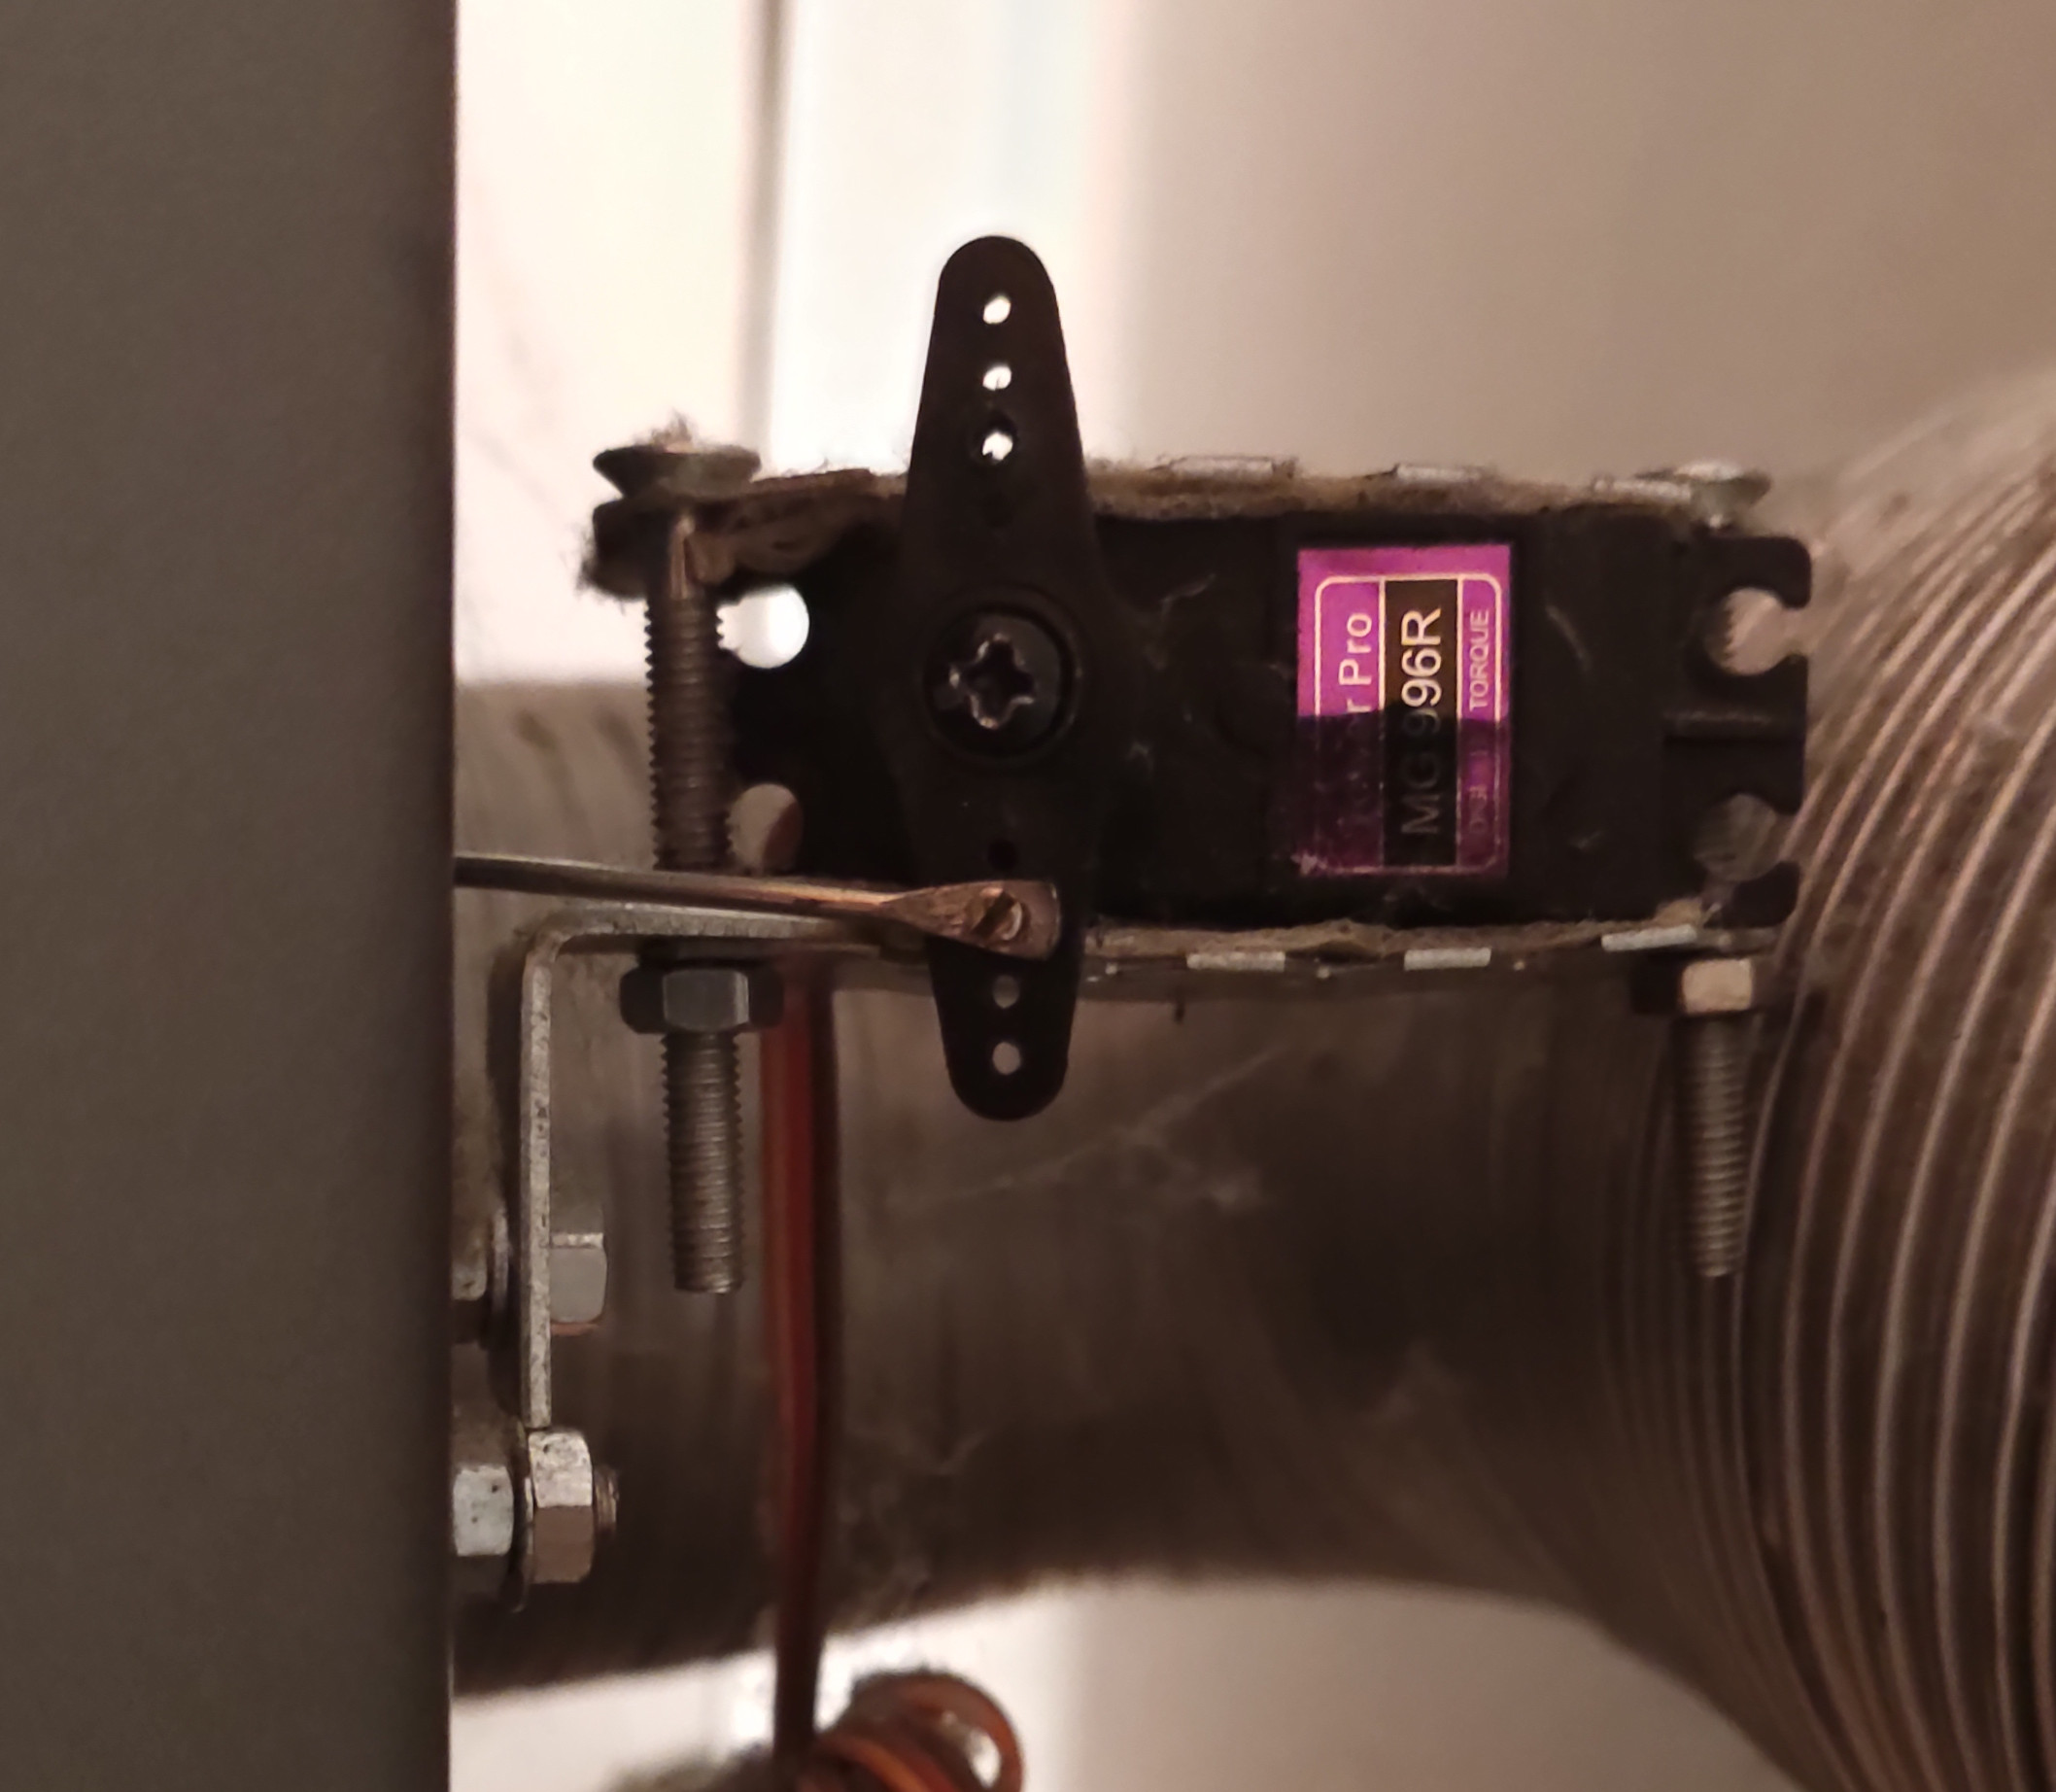
\includegraphics[width=0.8 \textwidth]{fig/servo.jpg}
\caption{Serwomechanizm zainstalowany przy piecu kominkowym. (opracowanie własne)}
\label{fig:servo}
\end{figure}
 
 \section{Moduł Ethernet}
 Zdecydowano się na dołączenie dodatkowego modułu Ethernet, ponieważ sterownik bez przerwy komunikuje się z siecią w celu wymiany informacji. Wykorzystanie komunikacji WiFi generowałoby niepotrzebny smog elektromagnetyczny. Wybrany moduł W5500 Lite jest nieznacznie droższy, ale za to bardziej kompaktowy niż inne rozwiązania oparte o układ W5500.
 
 \section{Zegar czasu rzeczywistego}
 Pierwotnie planowano wykorzystać moduł czasu rzeczywistego z podtrzymaniem. Jednakże, sterownik przez większość czasu będzie podłączony do internetu, skąd może pozyskać aktualną godzinę, dlatego zrezygnowano z tego rozwiązania.
 
 \section{Urządzenie wskazujące}
 Pierwszym planowanym rozwiązaniem było wykorzystanie przycisków typu pushbutton. Mikrokontroler ESP32 posiada jednak specjalne piny umożliwiające rozpoznawanie dotyku poprzez detekcję zmian pojemności, dlatego zdecydowano się zastąpić pushbuttony panelem dotykowym.
 
 \section{Czujnik otwarcia drzwi paleniska}
 Czujnik otwarcia drzwi paleniska pozwala na wykrywanie momentów dokładania paliwa. W projekcie wykorzystano prosty przełącznik podłączony do pinu cyfrowego mikrokontrolera.
 
 \section{Zasilanie awaryjne}
 Najprostszym z rozważanych rozwiązań było zastosowanie dodatkowego, zewnętrznego modułu typu powerbank. Jednak jego wykorzystanie nie dawałoby żadnej kontroli nad trybem zasilania sterownika, co mogłoby skutkować nagłym przerwaniem dostaw energii, a w konsekwencji możliwością przegrzania pieca. Wybrano płytkę rozszerzeń typu battery shield z dwoma akumulatorami litowo-jonowymi 18650 o pojemności około 3600mAh każdy oraz układem ładowania i układem zabezpieczającym przed całkowitym rozładowaniem.
 
 \section{Źródło dźwięku}
 Jako źródło dźwięku w projekcie wykorzystano brzęczyk pasywny. W odróżnieniu od aktywnego, umożliwia on generowanie dźwięków o zmiennej częstotliwości za pomocą sygnału PWM. Dla ułatwienia konstrukcji zdecydowano się wybrać moduł brzęczyka zawierający tranzystor sterujący, który chroni źródło sygnału przed przeciążeniem prądowym.
 
 \section{Rodzaj połączenia czujników zewnętrznych}
 Ze względu na łatwość i pewność połączenia zdecydowano się na wybranie standardu złącza 8P8C, wykorzystywanego w rożnego rodzaju sprzęcie telekomunikacyjnym i komputerowym. Jest ono rozpowszechnione jako złącze do budowy sieci w standardzie Ethernet. 8P8C to złącze o ośmiu miejscach na styk i ośmiu stykach.
 
 
 \chapter[Wykonanie prototypu sterownika pieca kominkowego\\ na płytce stykowej]{Wykonanie prototypu sterownika pieca kominkowego na płytce stykowej}\label{ch:prototyp:stykowa}
 \chaptermark{Prototyp na płytce stykowej}
 W tym rozdziale opisany został proces prototypowania z wykorzystaniem płytki stykowej.
 Pozwala ona na łatwe połączenie elementów tworzonego układu. Podzespoły wpinane są w płytkę, a następnie łączone elektrycznie przy pomocy specjalnych przewodów.
 Pierwszym elementem sterownika umieszczonym na płytce był mikrokontroler ESP32. Nie wymagał on dodatkowych połączeń, ponieważ może być zasilany przez port USB.
    Zdjęcie~\ref{fig:stykowa} przedstawia płytkę stykową z podłączonymi modułami sterownika pieca kominkowego.
    \begin{figure}[ht]
\centering
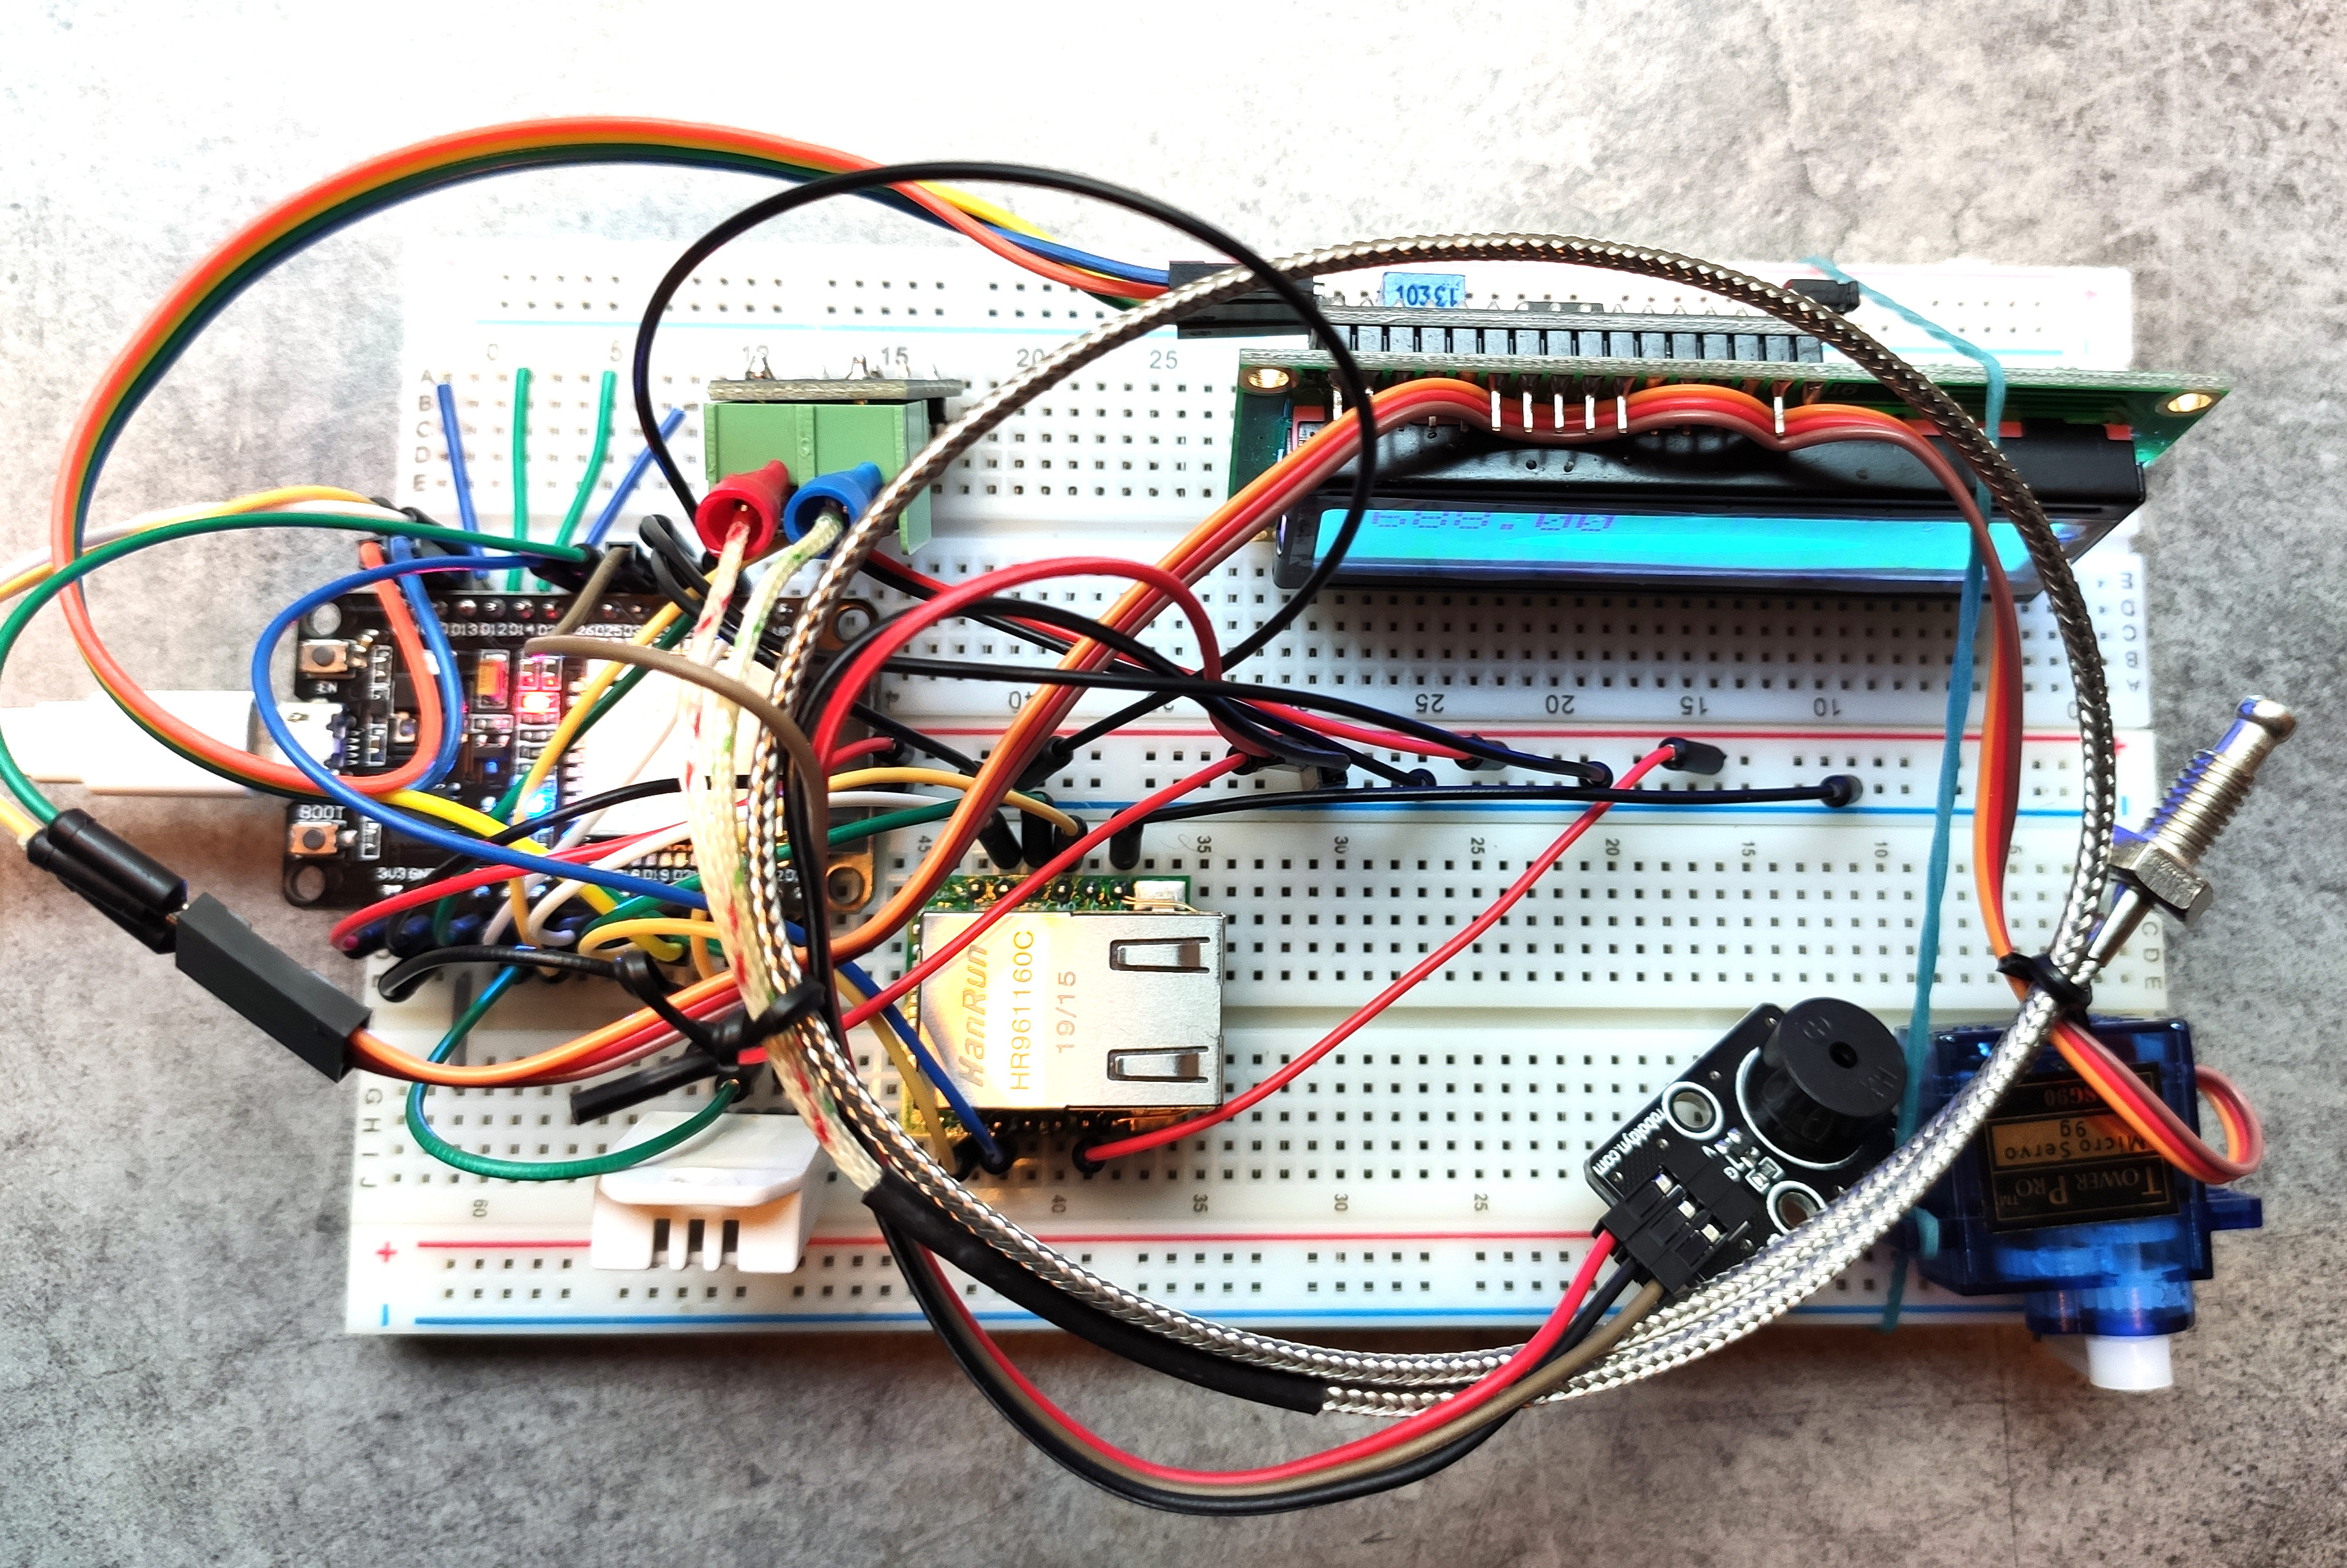
\includegraphics[width=0.8 \textwidth]{fig/plytka_stykowa.jpg}
\caption{Płytka stykowa z podłączonymi modułami. (opracowanie własne)}
\label{fig:stykowa}
\end{figure}
  
 \section{Połączenie mikrokontrolera oraz LCD}
 Użyty w projekcie wyświetlacz LCD 16x2 posiada dodatkowo konwerter I2C, który zmniejsza ilość linii niezbędnych do komunikacji z 16 do 4. Wykorzystana do komunikacji magistrala I2C jest szeregowa oraz dwukierunkowa. Wykorzystuje tylko dwie linie komunikacyjne - Serial Data i Serial Clock. Transfer danych może być zainicjowany tylko, gdy magistrala nie jest zajęta. Poza liniami transferu danych wyświetlacz potrzebuje także pary linii zasilania - masy oraz 5V.
  
 \section{Podłączenie termometru i czujnika wilgotności DHT22}\label{dht}
 Do komunikacji z mikrokontrolerem moduł termometru i czujnika wilgotności DHT22  używa magistrali 1-Wire, która wykorzystuje pojedynczą linię komunikacyjną. W zależności od długości przewodów należy wybrać właściwy rezystor podciągający.  Mikrokontroler ESP32 posiada wbudowany opornik podciągający o wartości około 50k Ohmów. Jeśli przewody przyłączeniowe nie są długie, wtedy nie ma potrzeby wykorzystywania dodatkowego rezystora.
 Moduł termometru DHT22 potrzebuje również zasilania 3,3V.
 
 \section{Podłączenie termometru Dallas}
 Układ termometru Dallas DS18B20, do komunikacji z mikrokontrolerem, wykorzystuje magistrale 1-Wire opisaną w części \ref{dht}. Dodatkowo potrzebuje zasilania 3,3V.
 
 \section{Podłączenie układu MAX6675 - termopara}
 Układ MAX6675 wykorzystuje do komunikacji magistralę SPI, posiadającą trzy linie komunikacyjne: SO - Master Input Slave Output, CS - Chip Select, SCK - Serial Clock. Do zasilania układu potrzebne jest zasilanie 3,3V.
 
 \section{Podłączenie serwomechanizmu}
 Do podłączenia serwomechanizmu wystarczy jedna linia komunikacyjna przesyłająca sygnał PWM oraz zasilanie 5V.
 
 \section{Podłączenie czujnika otwarcia paleniska}
 Czujnik otwarcia drzwi paleniska, w postaci prostego przełącznika, został podłączony do pinu cyfrowego mikrokontrolera pojedynczą linią komunikacyjną. Linia ta będzie ustawiana w stan wysoki przy pomocy rezystora podciągającego. Otwarcie drzwi spowoduje zwarcie linii do masy. 
 
  \section{Podłączenie układu Ethernet W5500 Light}
 Moduł W5500 wykorzystuje do komunikacji magistralę SPI, posiadającą 4 linie komunikacyjne: MO - Master Output Slave Input, SO - Master Input Slave Output ,CS - Chip Select, SCK - Serial Clock.
 Podczas podłączania układu napotkano problemy z komunikacją. Konieczna była zmiana wykorzystywanych pinów mikrokontrolera.
 
 \section{Podłączenie brzęczyka}
 Do podłączenia brzęczyka potrzebna jest jedna linia komunikacyjna przesyłająca sygnał PWM oraz zasilanie 5V. 
 Podczas podłączania natknięto się na błędy komunikacyjne. Przyczyną okazało się błędne nazewnictwo pinów. Pin 32 został zamieniony z pinem 33 w opisie wyprowadzeń na płytce deweloperskiej mikrokontrolera ESP32.
 
 
 \section{Wykonanie okablowania}
 Podłączenie zewnętrznych czujników do sterownika wykonałem z wykorzystaniem skrętki ekranowanej, która zapewnia odporność komunikacji na zakłócenia transmisji.
 
 
 \chapter{Opracowanie oprogramowania -~część pierwsza}\label{ch:oprog:1}
  \chaptermark{Opracowanie oprogramowania I}
 W tym rozdziale opisano proces opracowywania pierwszej części oprogramowania, stanowiącej podstawę komunikacji z modułami sterownika. Dalsza część procesu programowania została opisana w rozdziale \ref{ch:oprog:2}.
 
 \section{Utworzenie projektu}
 Do programowania sterownika wykorzystano środowisko programistyczne CLion wraz z ekosystemem PlatformIO.
 CLion to wieloplatformowe zintegrowane środowisko programistyczne (IDE) przeznaczone dla języków C/C++.
 PlatformIO Core jest sercem całego ekosystemu PlatformIO ułatwiającego programowanie mikrokontrolerów. Dostarcza interfejs wiersza poleceń. PlatformIO Core napisana jest w języku Python.
 Projekt oprogramowania sterownika został zainicjowany w pustym katalogu poleceniem:
 \begin{lstlisting}
platformio init --ide clion --board esp32doit-devkit-v1 
 \end{lstlisting}
 Definiuje ono z jakiego IDE chcemy skorzystać oraz jaki mikrokontroler będzie programowany.
 Następnie projekt został otwarty w CLion, gdzie przebiega dalszy proces programowania.
 
 \section{Edycja pliku konfiguracyjnego projektu}
 W celu zmiany konfiguracji projektu należy poddać edycji plik platformio.ini. Daje on przede wszystkim możliwość wybrania frameworka, dodatkowych bibliotek, prędkości komunikacji z mikrokontrolerem przez monitor portu szeregowego oraz parametrów wgrywania oprogramowania do mikrokontrolera.
 
 \section{Szkielet do budowy aplikacji}
 Spośród dwóch dostępnych dla mikrokontrolera ESP32 frameworków, ze względu na dużą ilość gotowych bibliotek do komunikacji z modułami, zdecydowano się na wykorzystanie platformy programistycznej Arduino.
 Program napisany dla tej platformy musi posiadać plik main, w którym są dwie funkcje: setup oraz loop.
 Setup wykonywany jest tylko raz po uruchomieniu mikrokontrolera, natomiast loop wykonuje się w nieskończonej pętli aż do momentu zakończenia pracy.
 
 \section{Dodanie bibliotek i podstawowa komunikacja z urządzeniami}
 Pisanie oprogramowania rozpoczęto od dodania bibliotek pozwalających na komunikację z urządzeniami, aby sprawdzić poprawność działania prototypu wykonanego na płytce stykowej. Dla każdego urządzenia stworzono osobny plik .h zawierający deklaracje funkcji oraz plik .cpp zawierający ich definicje.
 W dalszej kolejności zostało opisane użycie poszczególnych bibliotek.
  \subsection{Dodanie portalu przechwytującego}
 Pierwszym krokiem, umożliwiającym łatwą konfigurację połączenia Wi-Fi w sterowniku, było wykorzystanie biblioteki ESP Acync WiFiManager \cite{WiFiManager}, która pozwala na automatyczne tworzenie sieci WiFi ad-hoc i portalu przechwytującego. Daje to możliwość wyboru oraz połączenia się z docelową siecią WiFi, zapewniającą łączność sterownika z Internetem.
 Dla utworzenia WiFi Menagera należy konstruktorowi przekazać dwa obiekty: serwer web oraz server dns. Następnie powinno się zdefiniować funkcję zwrotną (callback) wykonywaną w momencie utworzenia przez WiFi Manger punktu dostępowego. Aby uruchomić Menagerera należy wywołać metodę autoConnect, przekazując jej, jako opcjonalne parametry, nazwę tworzonego acces pointa oraz hasło. Po uruchomieniu Menager próbuje się połączyć z poprzednio zapamiętaną siecią WiFi. Jeśli jej nie odnajdzie, tworzy punkt dostępowy oraz portal przechwytujący, w którym można wybrać inną sieć.
 \subsection{Dodanie biblioteki dla DHT22}
 Do komunikacji z czujnikiem temperatury i wilgotności wykorzystano bibliotekę DHT sensor library for ESPx \cite{DHTlibrary}. Aby zainicjować działanie biblioteki należy skorzystać z metody setup podając jako parametry numer pinu, do którego podłączony jest czujnik, oraz model czujnika. Do odczytania pomiarów służą metody getTemperature oraz getHumididity.
 \subsection{Dodanie biblioteki dla MAX6675}
 Do komunikacji z termoparą w projekcie wykorzystano bibliotekę MAX6675 library \cite{MAX6675library}. Aby zainicjować moduł należy skorzystać z konstruktora, przekazując jako parametry numery pinów używanych do komunikacji z magistralą SPI.
 W celu odczytania temperatury należy skorzystać z metody readCelsius.
 \subsection{Dodanie biblioteki dla LCD}
 Do komunikacji z wyświetlaczem LCD, przy udziale magistrali I2C, wykorzystałem bibliotekę LiquidCrystal PCF8574 \cite{LCDlibrary}. Adres wyświetlacza na magistrali, przekazany jako argument konstruktora pozwala zainicjować bibliotekę. Metoda setBacklight pozwala na włączenie podświetlenia wyświetlacza. Do wypisywania tekstu na wyświetlaczu służą metody print oraz println.
 \subsection{Dodanie biblioteki dla serwomechanizmu}
 Do komunikacji z serwomechanizmem wykorzystano bibliotekę ESP32Servo \cite{Servolibrary}. Aby rozpocząć pracę należy skorzystać z metody attach, podając jako argument numer pinu będącego wyjściem sygnałowym. W celu ustawienia mechanizmu na wybraną pozycję należy skorzystać z metody write. Metoda detach służy do przerwania komunikacji z serwomechanizmem.
 \subsection{Dodanie biblioteki dla PID}
 Do sterowania wychyleniem serwomechanizmu posłużono się biblioteką PID \cite{PIDlibrary}. Pozwala ona na wykorzystanie regulatora proporcjonalno-całkująco-różniczkującego do utrzymywania wartości wyjściowej na zadanym poziomie.
 Aby zainicjować bibliotekę  należy skorzystać z konstruktora, przekazując jako parametr referencje do wartości wejściowej, wyjściowej, zadanej oraz trzy parametry regulatora. Przy pomocy funkcji SetSampleTime należy ustalić jak często regulator ma obliczać wartość wyjściową. Funkcja SetOutputLimits służy do określenia granic parametru wyjściowego. Natomiast funkcja SetControlDirection określa kierunek sprzężenia wejścia z wyjściem. Funkcja SetMode(AUTOMATIC) uruchamia działanie regulatora.
 \subsection{Dodanie biblioteki dla DS18B20}
 Do komunikacji z termometrem Dallas wykorzystano bibliotekę DallasTemperature \cite{dallaslibrary}. Aby zainicjować bibliotekę należy skorzystać z konstruktora, przekazując jako parametr referencję do obiektu oneWire. W celu odczytania temperatury należy skorzystać z metody requestTemperatures, a następnie getTempCByIndex.
 \subsection{Dodanie biblioteki dla W5500 Light}
 Do komunikacji z modułem W5500 Light wykorzystano bibliotekę Ethernet Library for Arduino \cite{ethernetlibrary}. Aby zainicjować bibliotekę należy użyć metody init, podając jako parametr numer pinu Chip Select. Następnie należy skorzystać z metody WizReset wykonującej sekwencję resetowania modułu. W celu rozpoczęcia połączenia Ethernetowego należy użyć metody begin, podając jako parametry adres MAC, adres IP, adres DNS, adres bramy oraz maskę.
 \subsection{Dodanie biblioteki WebThings}
 Do przekształcenia sterownika w rzecz webową wykorzystano bibliotekę webthing-arduino \cite{webthinglibrary}. Tworzy ona prosty serwer implementujący Web of Things API.
 Aby zainicjować bibliotekę należy skorzystać z konstruktora, przekazując jako parametry nazwę oraz adres IP. Następnie należy utworzyć instancję urządzenia oraz dodać do niego jego właściwości. Aby rozpocząć pracę serwera należy skorzystać z metody begin. Do przekazywania wartości właściwości urządzenia służą metody setValue oraz update.
 
 \section{Dodanie możliwości zdalnego uaktualniania oprogramowania}
 Mechanizm Over The Air Update pozwala na wgrywanie nowych wersji oprogramowania przez sieć LAN lub Internet (jeśli urządzenie posiada publiczny adres IP). W celu uruchomieniu OTA należy, w pliku konfiguracyjnym projektu jako protokół wgrywania, wybrać espota, a następnie podać adres urządzenia. Dla zabezpieczenia przed nieuprawnioną zmianą oprogramowania należy ustawić hasło blokujące dostęp.
 
 \section{Dodanie odczytu napięć}
 Mikrokontroler ESP32 posiada dwa 12 bitowe przetworniki ADC, z których drugi nie może być używany, gdy wykorzystywane jest WiFi. Domyślna rozdzielczość, 12 bitów (0 – 4095), może być zmniejszona do 9 bitów (0 – 511).
 Przy pomocy metody pinMode można określić numer pinu oraz tryb pracy (INPUT). Następnie należy skorzystać z metody analogRead, aby odczytać wartości napięć pinów mikrokontrolera.
 
 \section{Dodanie wykrywania dotyku}
 Mikrokontroler ESP32 posiada wbudowane 10 pojemnościowych sensorów dotyku, ale wykorzystana w projekcie płytka deweloperska ma wyprowadzone ich tylko 9. Odczyt sensorów dotyku jest bardzo prosty - wystarczy użyć funkcji touchRead jako argument, podając numer pinu.
 
 \section{Dodanie obsługi brzęczyka}
 Do wytwarzania dźwięku brzęczyk potrzebuje sygnału PWM. Do generowania sygnału PWM, przez mikrokontroler, wykorzystano moduł LED Control z frameworka. W pierwszej kolejności należy skorzystać z funkcji ledcSetup, podając trzy argumenty: kanał, częstotliwość oraz rozdzielczość. Następnie, aby rozpocząć generowanie należy skorzystać z funkcji ledcAttachPin, podając dwa argumenty: numer pinu, do którego podłączone jest wejście sygnałowe brzęczyka oraz kanał.
 Aby zaprzestać generowania należy skorzystać z funkcji ledcWrite, podając dwa argumenty: kanał oraz 0 (cykl pracy).
 
 \section{Testowanie sterownika}
 Po każdym etapie dodawania kolejnych modułów projektu, działanie sterownika było testowane z wykorzystaniem monitora portu szeregowego poprzez odczytanie mierzonych przez sterownik wartości.

 
 \chapter[Wykonanie prototypu sterownika pieca kominkowego\\ na płytce uniwersalnej]{Wykonanie prototypu sterownika pieca kominkowego na płytce uniwersalnej}\label{ch:prototyp:uniwersalna}
  \chaptermark{Prototyp na płytce uniwersalnej}
 W tym rozdziale opisano przeniesienie prototypu z płytki stykowej na płytkę uniwersalną.
 Wykorzystanie płytki uniwersalnej pozwala na pewniejsze połączenie podzespołów układu, jednocześnie pozostawiając wciąż pewną elastyczność do zmian w projekcie, co umożliwia dalsze jego doskonalenie.
 Zdjęcie~\ref{fig:uni_gora} przedstawia płytkę uniwersalną z gniazdami i połączeniami.
\begin{figure}[ht]
\centering
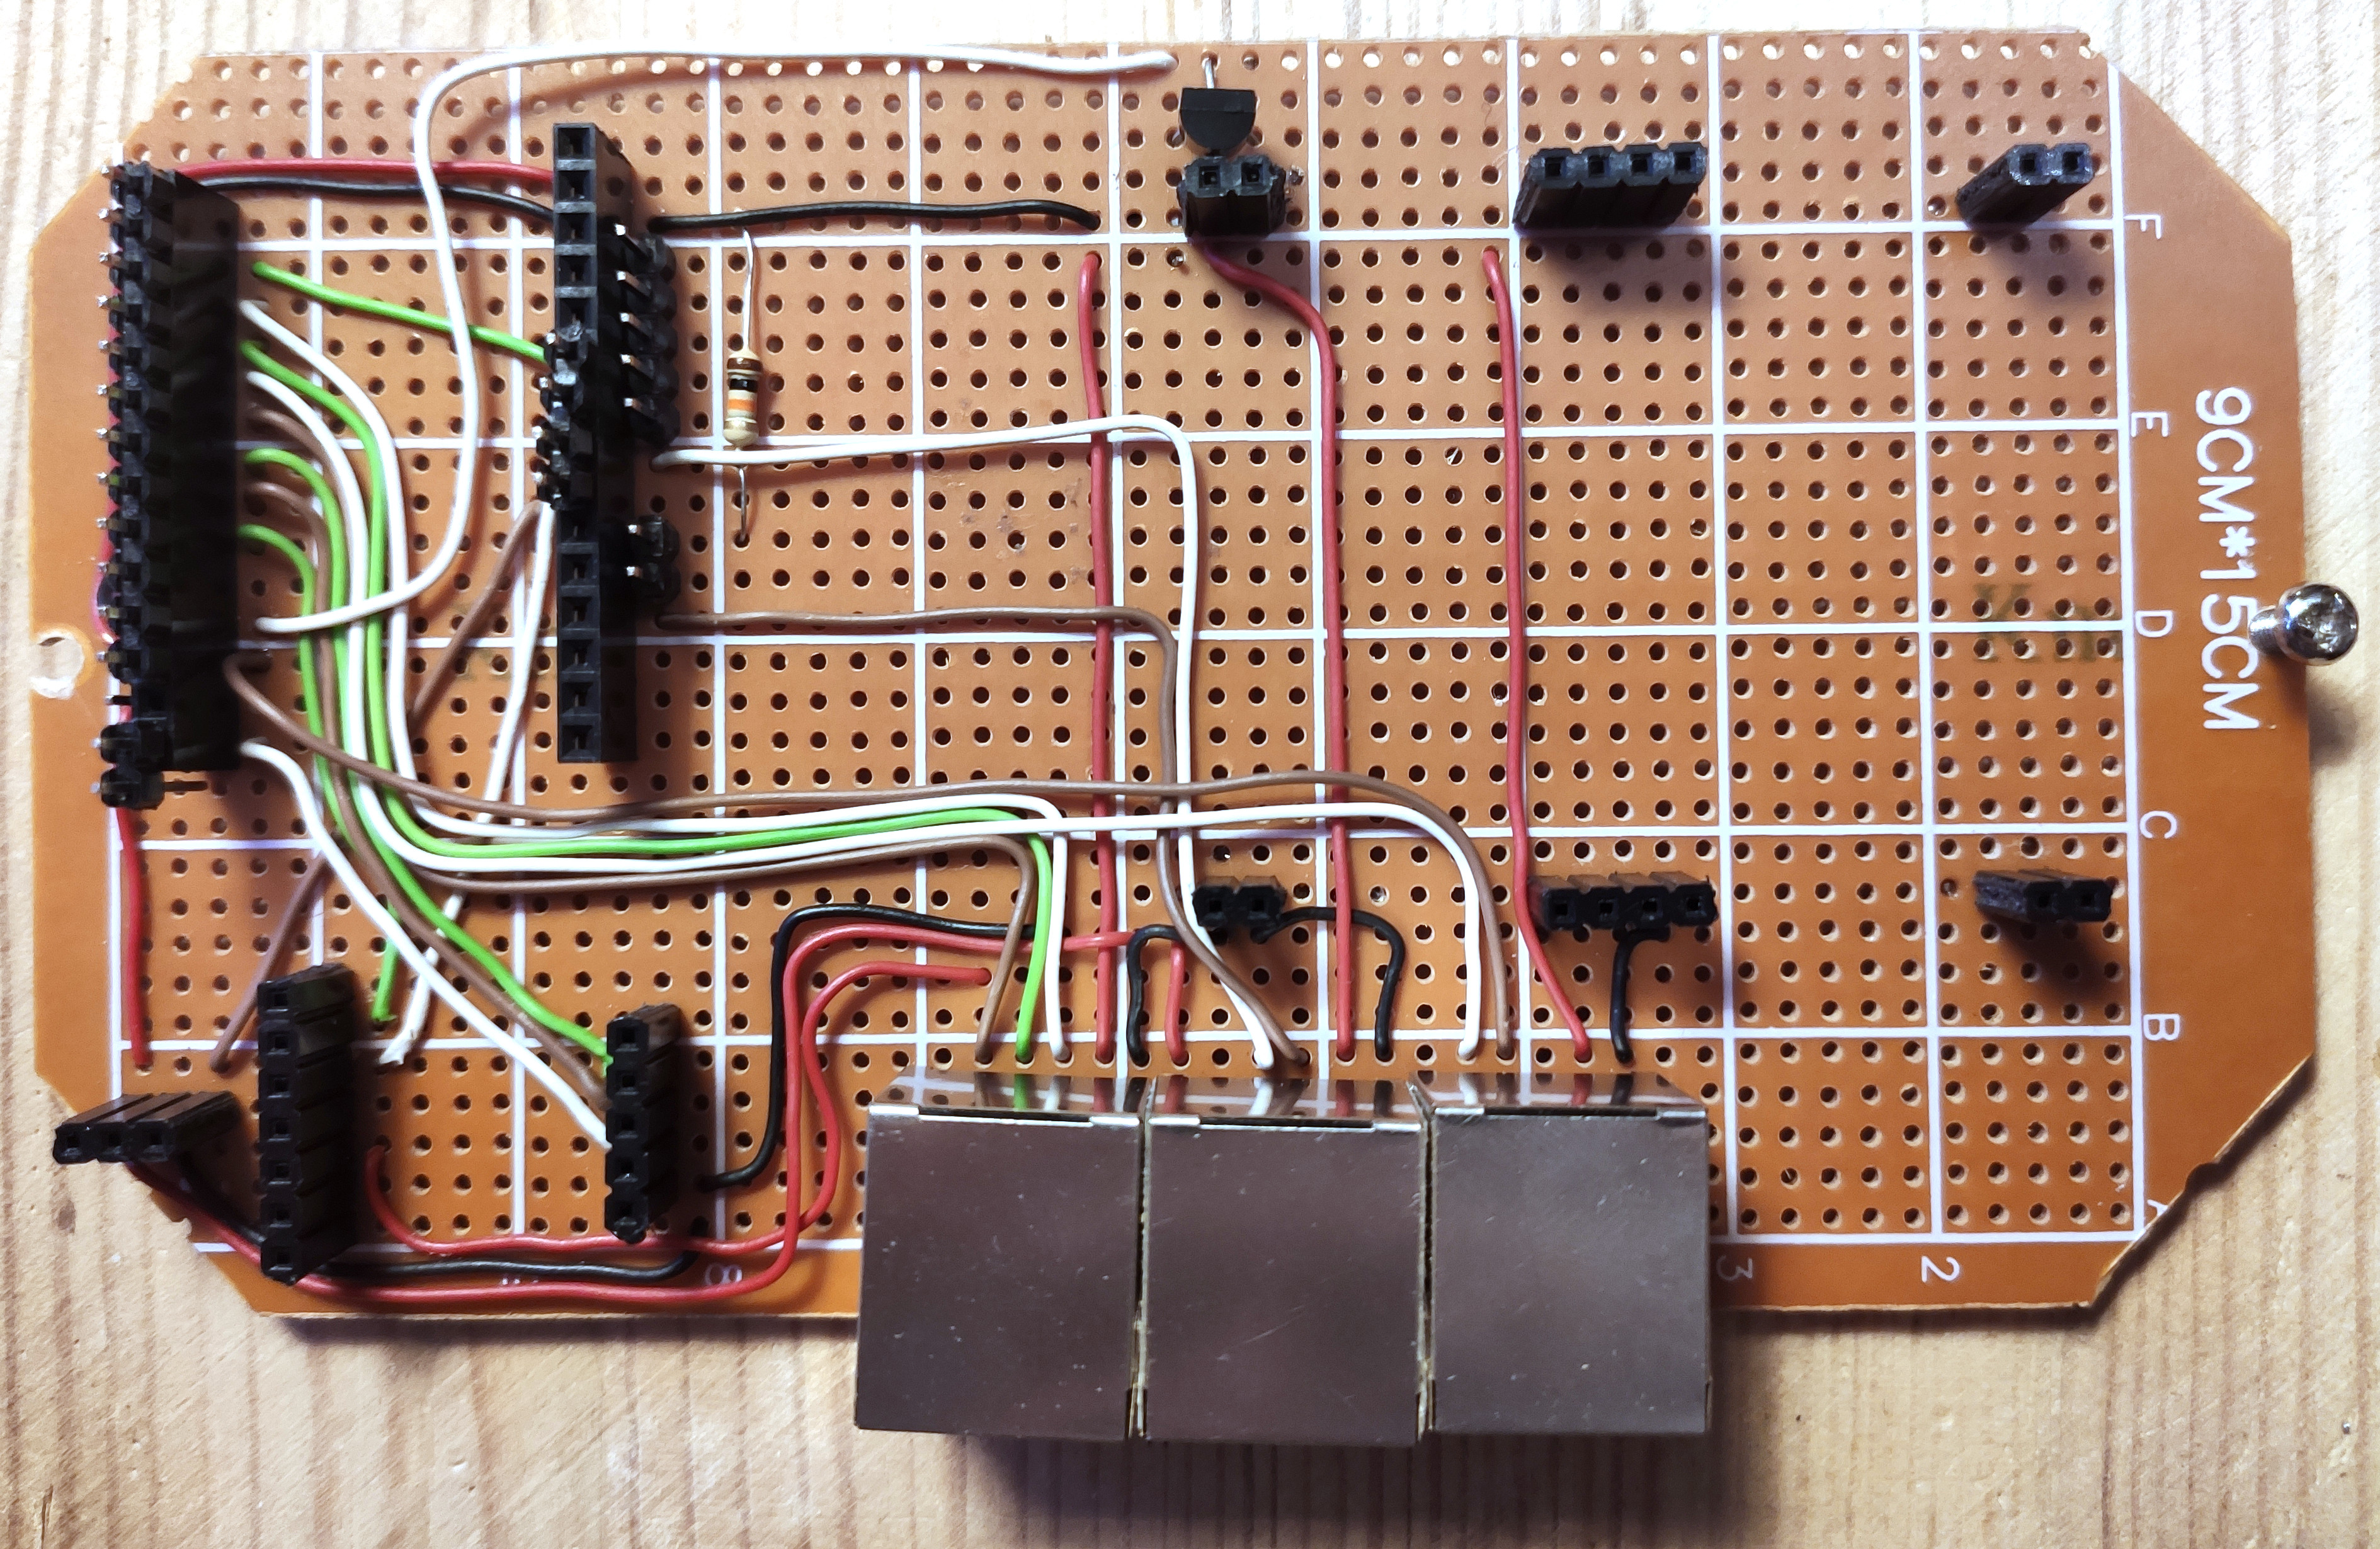
\includegraphics[width=0.8 \textwidth]{fig/plytka_gora.jpg}
\caption{Płytka uniwersalna z gniazdami i połączeniami. (opracowanie własne)}
\label{fig:uni_gora}
\end{figure}
 
 \section{Rozmieszczenie elementów}
 Dla wygodnego połączenia elementów wybrano płytkę uniwersalną o rozmiarach 9cm x 15cm ze standardowym rastrem otworów 2,54mm.
 Na początku na płytce umieszczono gniazda pod największe elementy: moduł zasilania o wymiarach 9,8cm x 2,9cm oraz mikrokontroler o wymiarach 5,5cm x 2,8cm. Gniazda pod kolejne elementy rozmieszczono tak, aby porty komunikacyjne oraz zasilania znajdowały się na dwóch krawędziach płytki. 
 Największą trudność sprawiło umieszczenie na płytce portów sieciowych, gdyż wyprowadzenie ich połączeń sygnałowych nie jest zgodne z rastrem 2,54mm, a dodatkowo potrzebne są otwory montażowe.
  
  \section{Wykonanie panelu dotykowego}
 Panel dotykowy wykonano z blaszek miedzianych o wymiarach 2cm x 2cm, przyklejonych do pokrywy sterownika, przylutowanych do przewodów zakończonych gniazdami. Podczas wycinania elementów należało zachować szczególną staranność dla zapewniania estetyki wykonania.
  Zdjęcie~\ref{fig:wieczko} przedstawia wieczko wraz z panelem dotykowym i wyświetlaczem LCD.
\begin{figure}[ht]
\centering
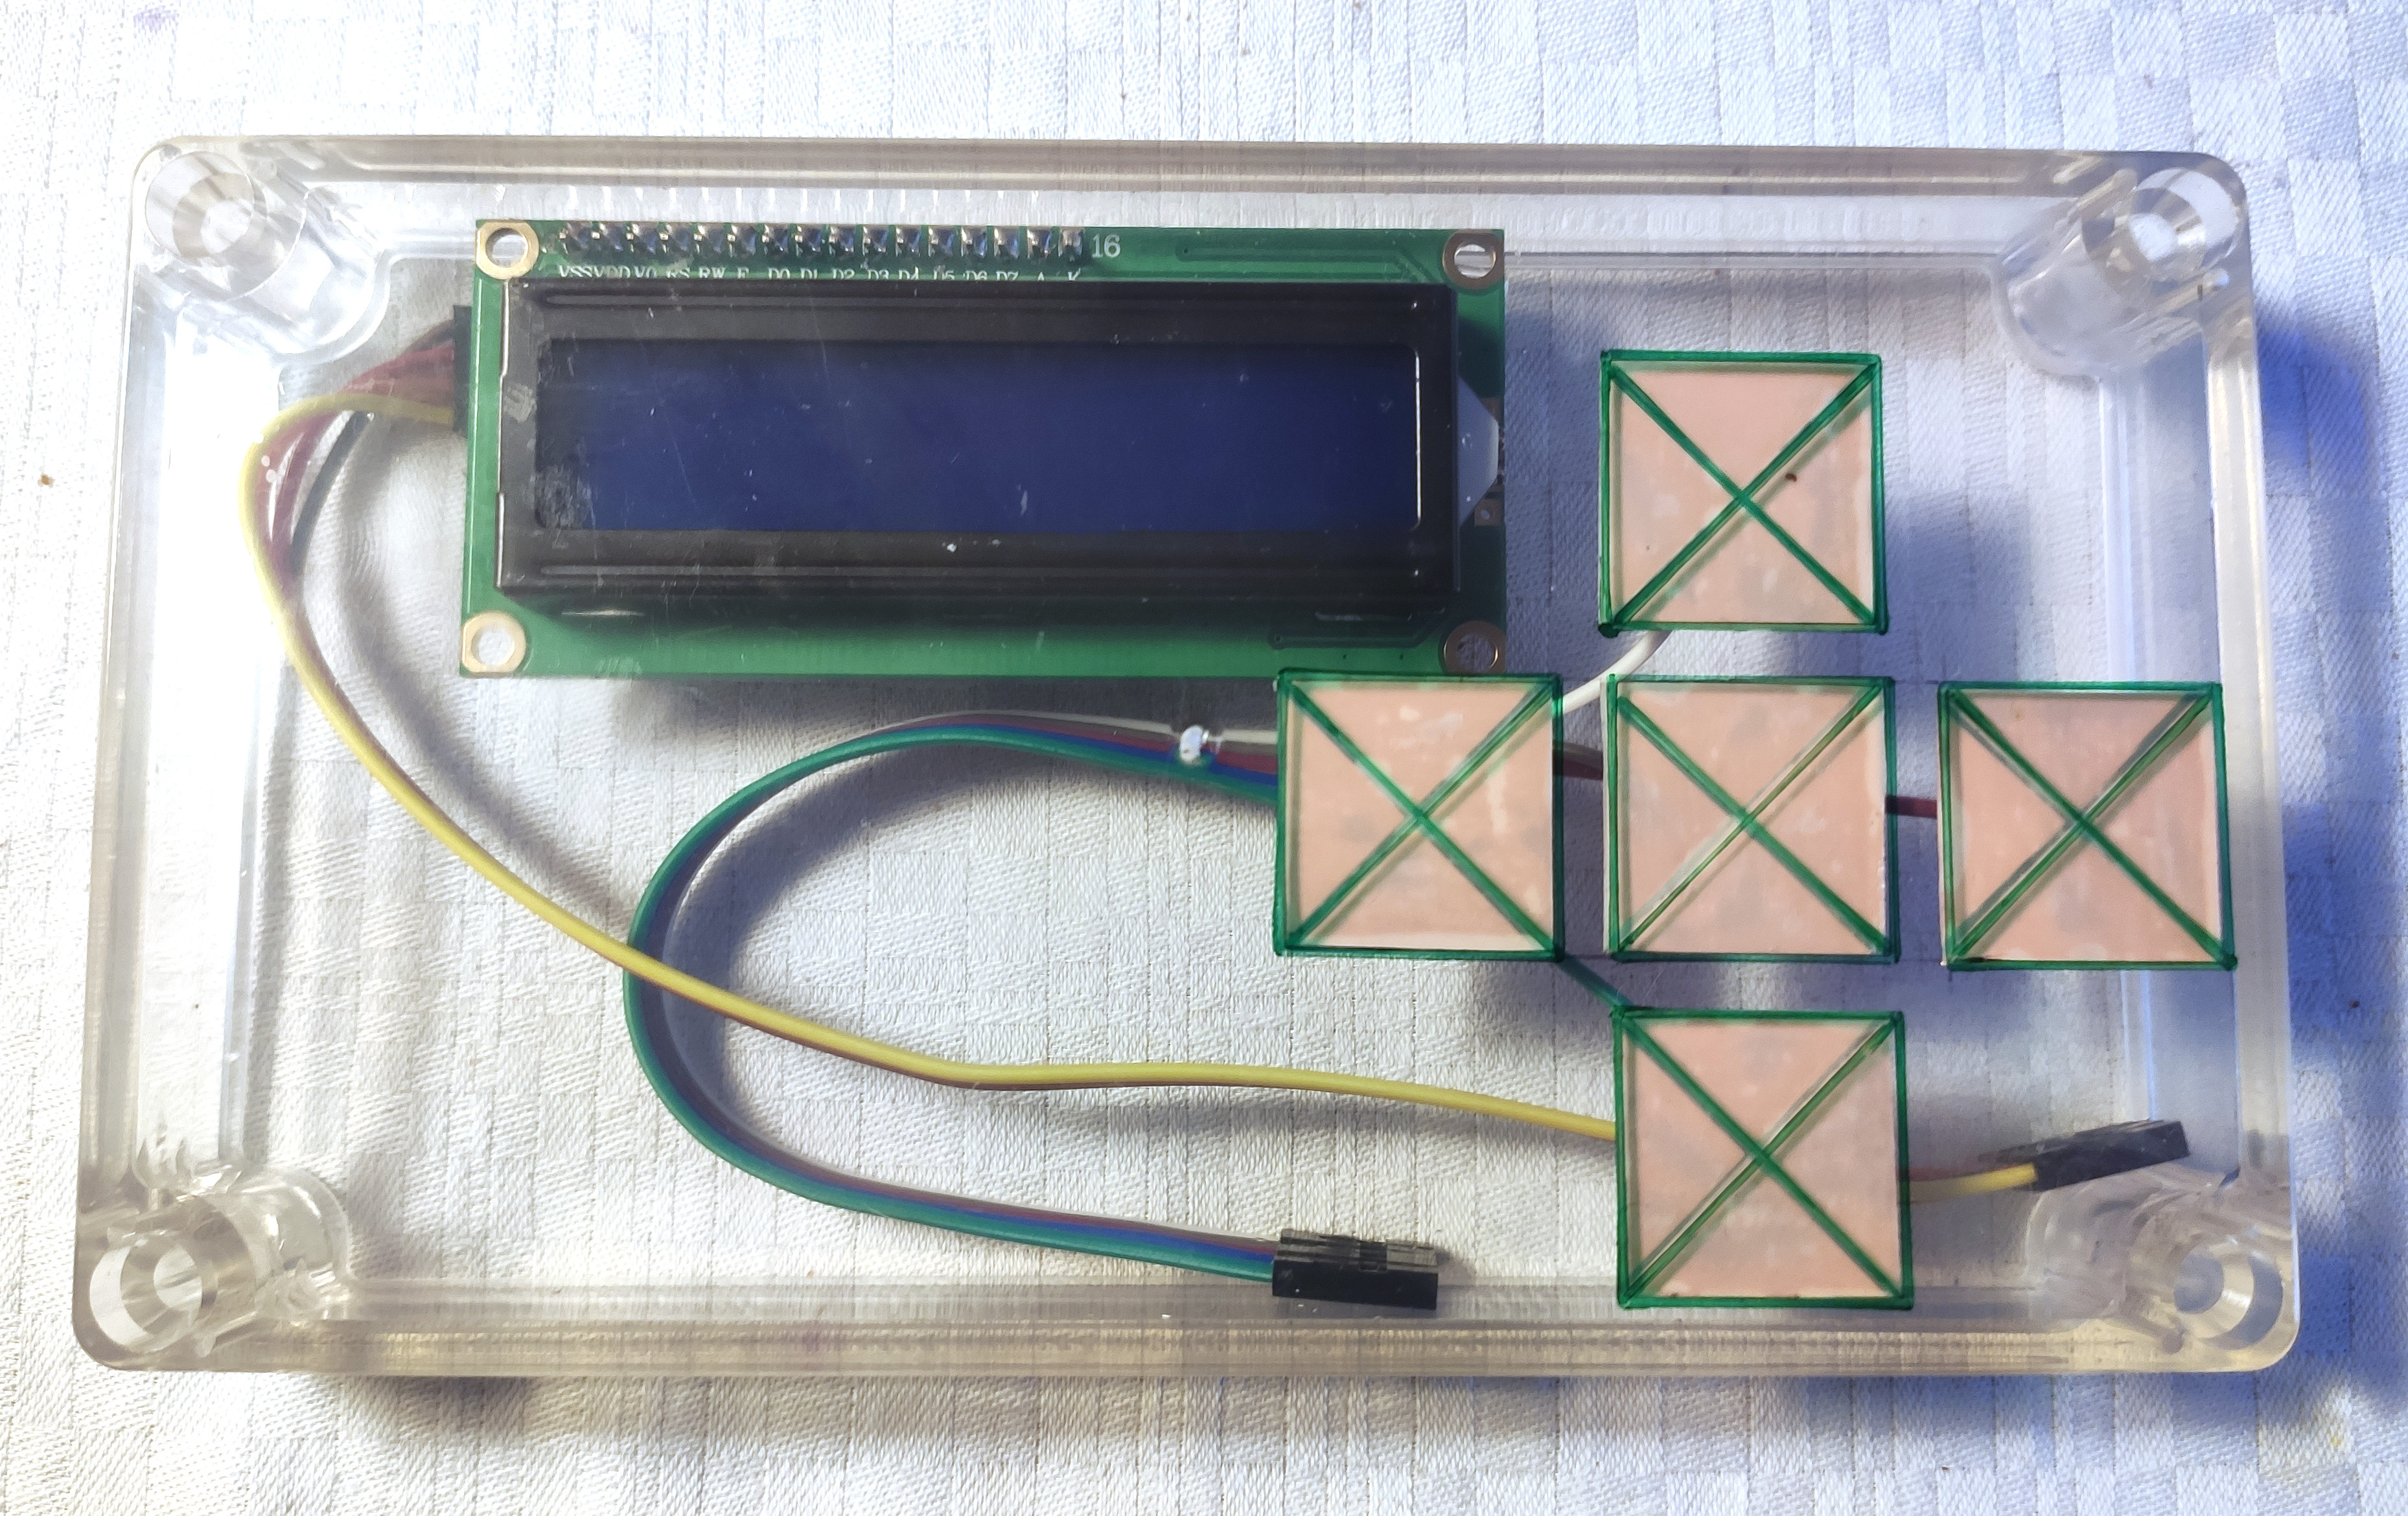
\includegraphics[width=0.8 \textwidth]{fig/wieczko.jpg}
\caption{Wieczko wraz z panelem dotykowym i wyświetlaczem LCD. (opracowanie własne)}
\label{fig:wieczko}
\end{figure}

 \section{Połączenie elementów}
 Gniazda oraz goldpiny wszystkich elementów zostały połączone jednożyłowymi przewodami miedzianymi w izolacji. Przewody rozmieszczono tak, aby łatwo można było prześledzić drogę połączenia, a następnie przylutowano je do płytki uniwersalnej. Różne kolory izolacji przewodów ułatwiają identyfikację połączeń. Zasilanie do złączy RJ-45 zostało doprowadzone tak, aby oba przewody znajdowały się w jednej parze skrętki, co pozwala na zmniejszenie ilości generowanych zakłóceń.
 Sprawdzenia poprawności połączeń dokonano przy pomocy miernika uniwersalnego.
   Zdjęcie~\ref{fig:uni_dol} przedstawia spodnią stronę płytki uniwersalnej z widocznymi połączeniami lutowanymi.
\begin{figure}[ht]
\centering
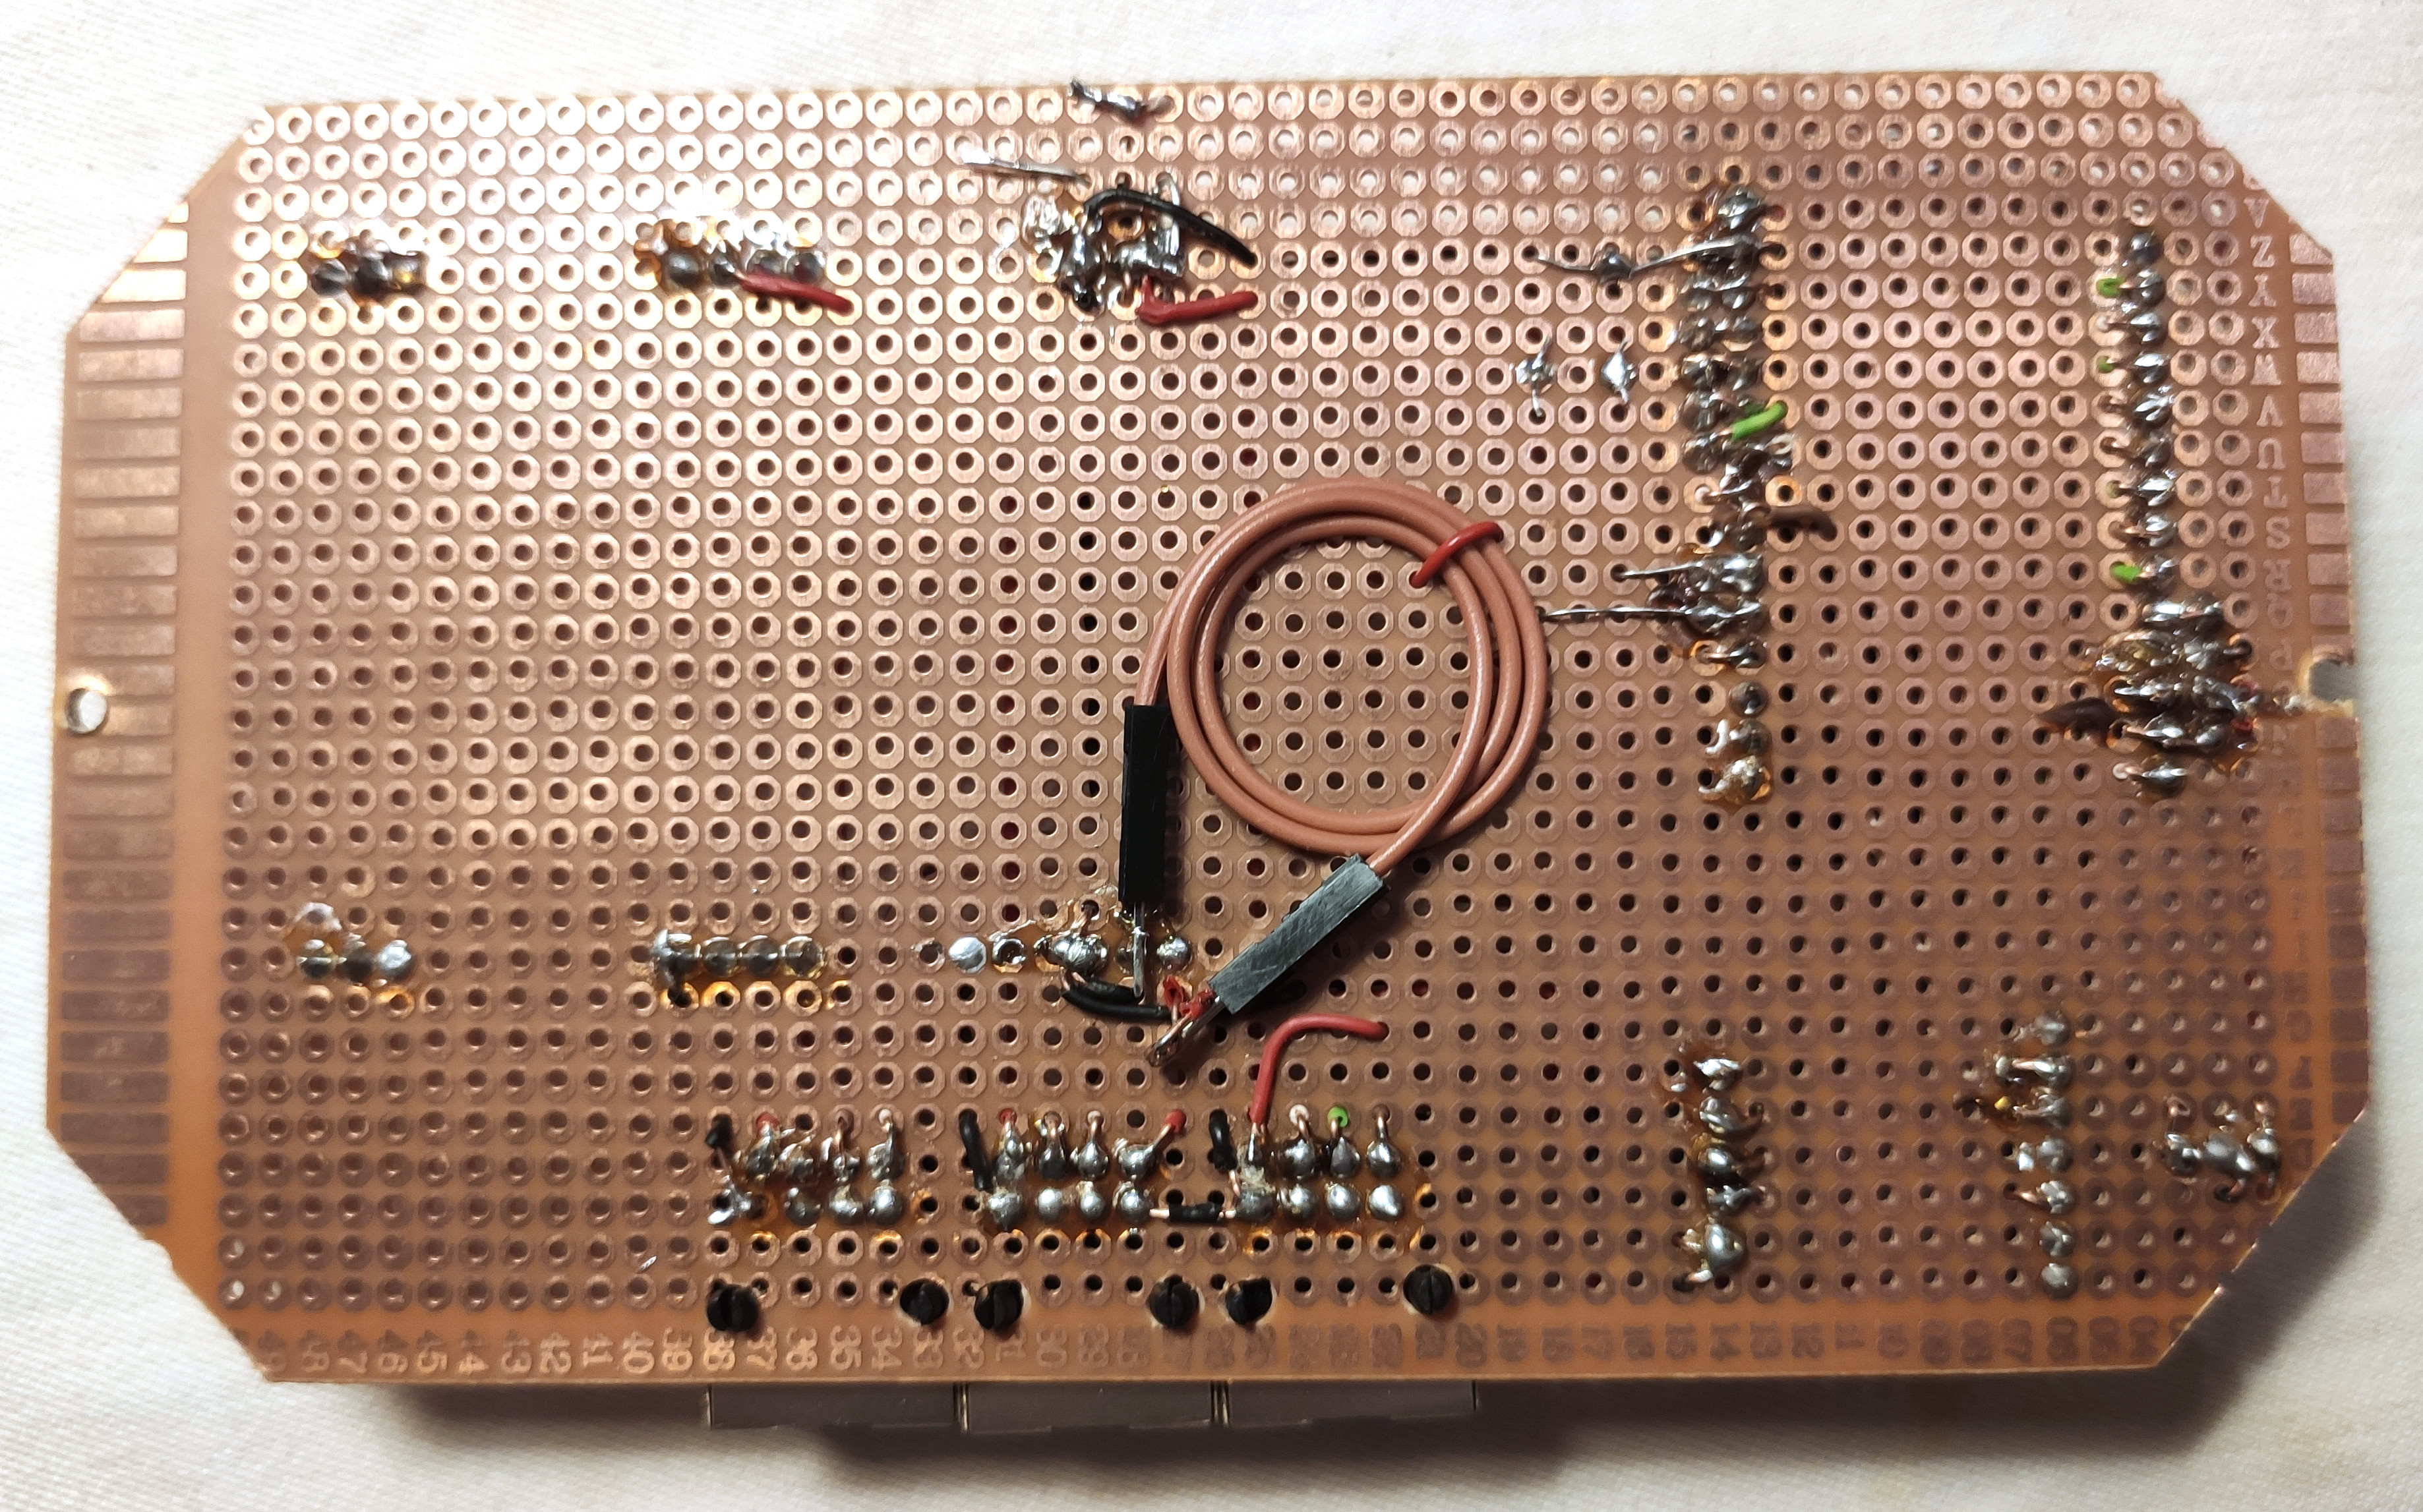
\includegraphics[width=0.8 \textwidth]{fig/plytka_dol.jpg}
\caption{Spodnia strona płytki uniwersalnej. (opracowanie własne)}
\label{fig:uni_dol}
\end{figure}

 \section{Zmiany w projekcie}
 Na etapie wykonywania prototypu na płytce uniwersalnej postanowiono wprowadzić kilka zmian do projektu sterownika.
 \subsection{Dodanie dzielnika napięcia}
 W celu wykrywania aktualnego źródła zasilania sterownika, zdecydowano się na pomiar napięcia zasilania diod sygnalizacyjnych w układzie modułu zasilania awaryjnego. Aby dostosować napięcia do zakresu bezpiecznego dla mikrokontrolera, zastosowano dzielniki napięcia składające się z rezystorów 1k Ohm.
 \subsection{Dodanie głównego włącznika zasilania}
 Dla umożliwienia łatwiejszego włączania zasilania zdecydowano się umieścić w projekcie dodatkowy przełącznik zasilania podłączony do modułu zasilania awaryjnego. Do małego przełącznika, znajdującego się w module zasilania, przylutowano dwa goldpiny. Duży przełącznik podłączono do przewodów zakończonych gniazdami szpilkowymi pasującymi do goldpinów.

 \section{Testowanie prototypu}
 Po podłączeniu wszystkich elementów sterownika do płytki uniwersalnej dokonano testu działania z wykorzystaniem monitora portu szeregowego.
 
 \chapter{Wykonanie obudowy}\label{ch:obudowa}
 Pierwotnie, w oparciu o pracę Francuza \cite{Frence2014} zamierzano wydrukować obudowę w  drukarce 3D. Jednak wielkość potrzebnej obudowy oraz czas niezbędny do wykonania projektu przesądziły o wykorzystaniu gotowej skrzynki, wykonanej z plastiku o przeźroczystym wieczku w rozmiarze 15,8cm x 9cm x 6cm, pozwalającej na swobodne zmieszczenie wszystkich komponentów sterownika. Płytka uniwersalna została przycięta na rogach, ponieważ obudowa posiada tam miejsca na śruby. W skrzynce wykonano 5 otworów: pierwszy na górnej powierzchni obudowy (względem docelowego umiejscowienia sterownika) na port micro USB, który jest przeznaczony na wypadek potrzeby bezpośredniego podłączenia do mikrokontrolera. Drugi na prawej płaszczyźnie, również na port micro USB, przeznaczony do zasilania podczas normalnej pracy. Natomiast na dolnej powierzchni obudowy znajdują się trzy otwory: z lewej strony wejście na gniazdo 8p8c, przeznaczone do połączenia z internetem. W środkowej części potrójne gniazdo 8p8c, służące do komunikacji z czujnikami zewnętrznymi oraz serwomechanizmem. Po prawej stronie znajduje się miejsce na główny włącznik.
 Po wykonaniu otworów i zamontowaniu komponentów sterownika przystąpiono do montowania panelu dotykowego. Poszczególne pola panelu zostały przyklejone do przezroczystego wieczka obudowy na kształt "+", każdy w odległości około 4mm od drugiego, co pozwala na minimalizację zakłóceń.
 Ostatnim etapem wykonania obudowy było wklejenie ekranu LCD, w lewym górnym rogu przeźroczystego wieczka sterownika.
 Po umieszczeniu w obudowie i podłączeniu wszystkich elementów sterownika dokonano testu działania z wykorzystaniem monitora portu szeregowego.
   Zdjęcie~\ref{fig:wnetrze} przedstawia spodnią część obudowy wraz z komponentami sterownika pieca kominkowego.
\begin{figure}[ht]
\centering
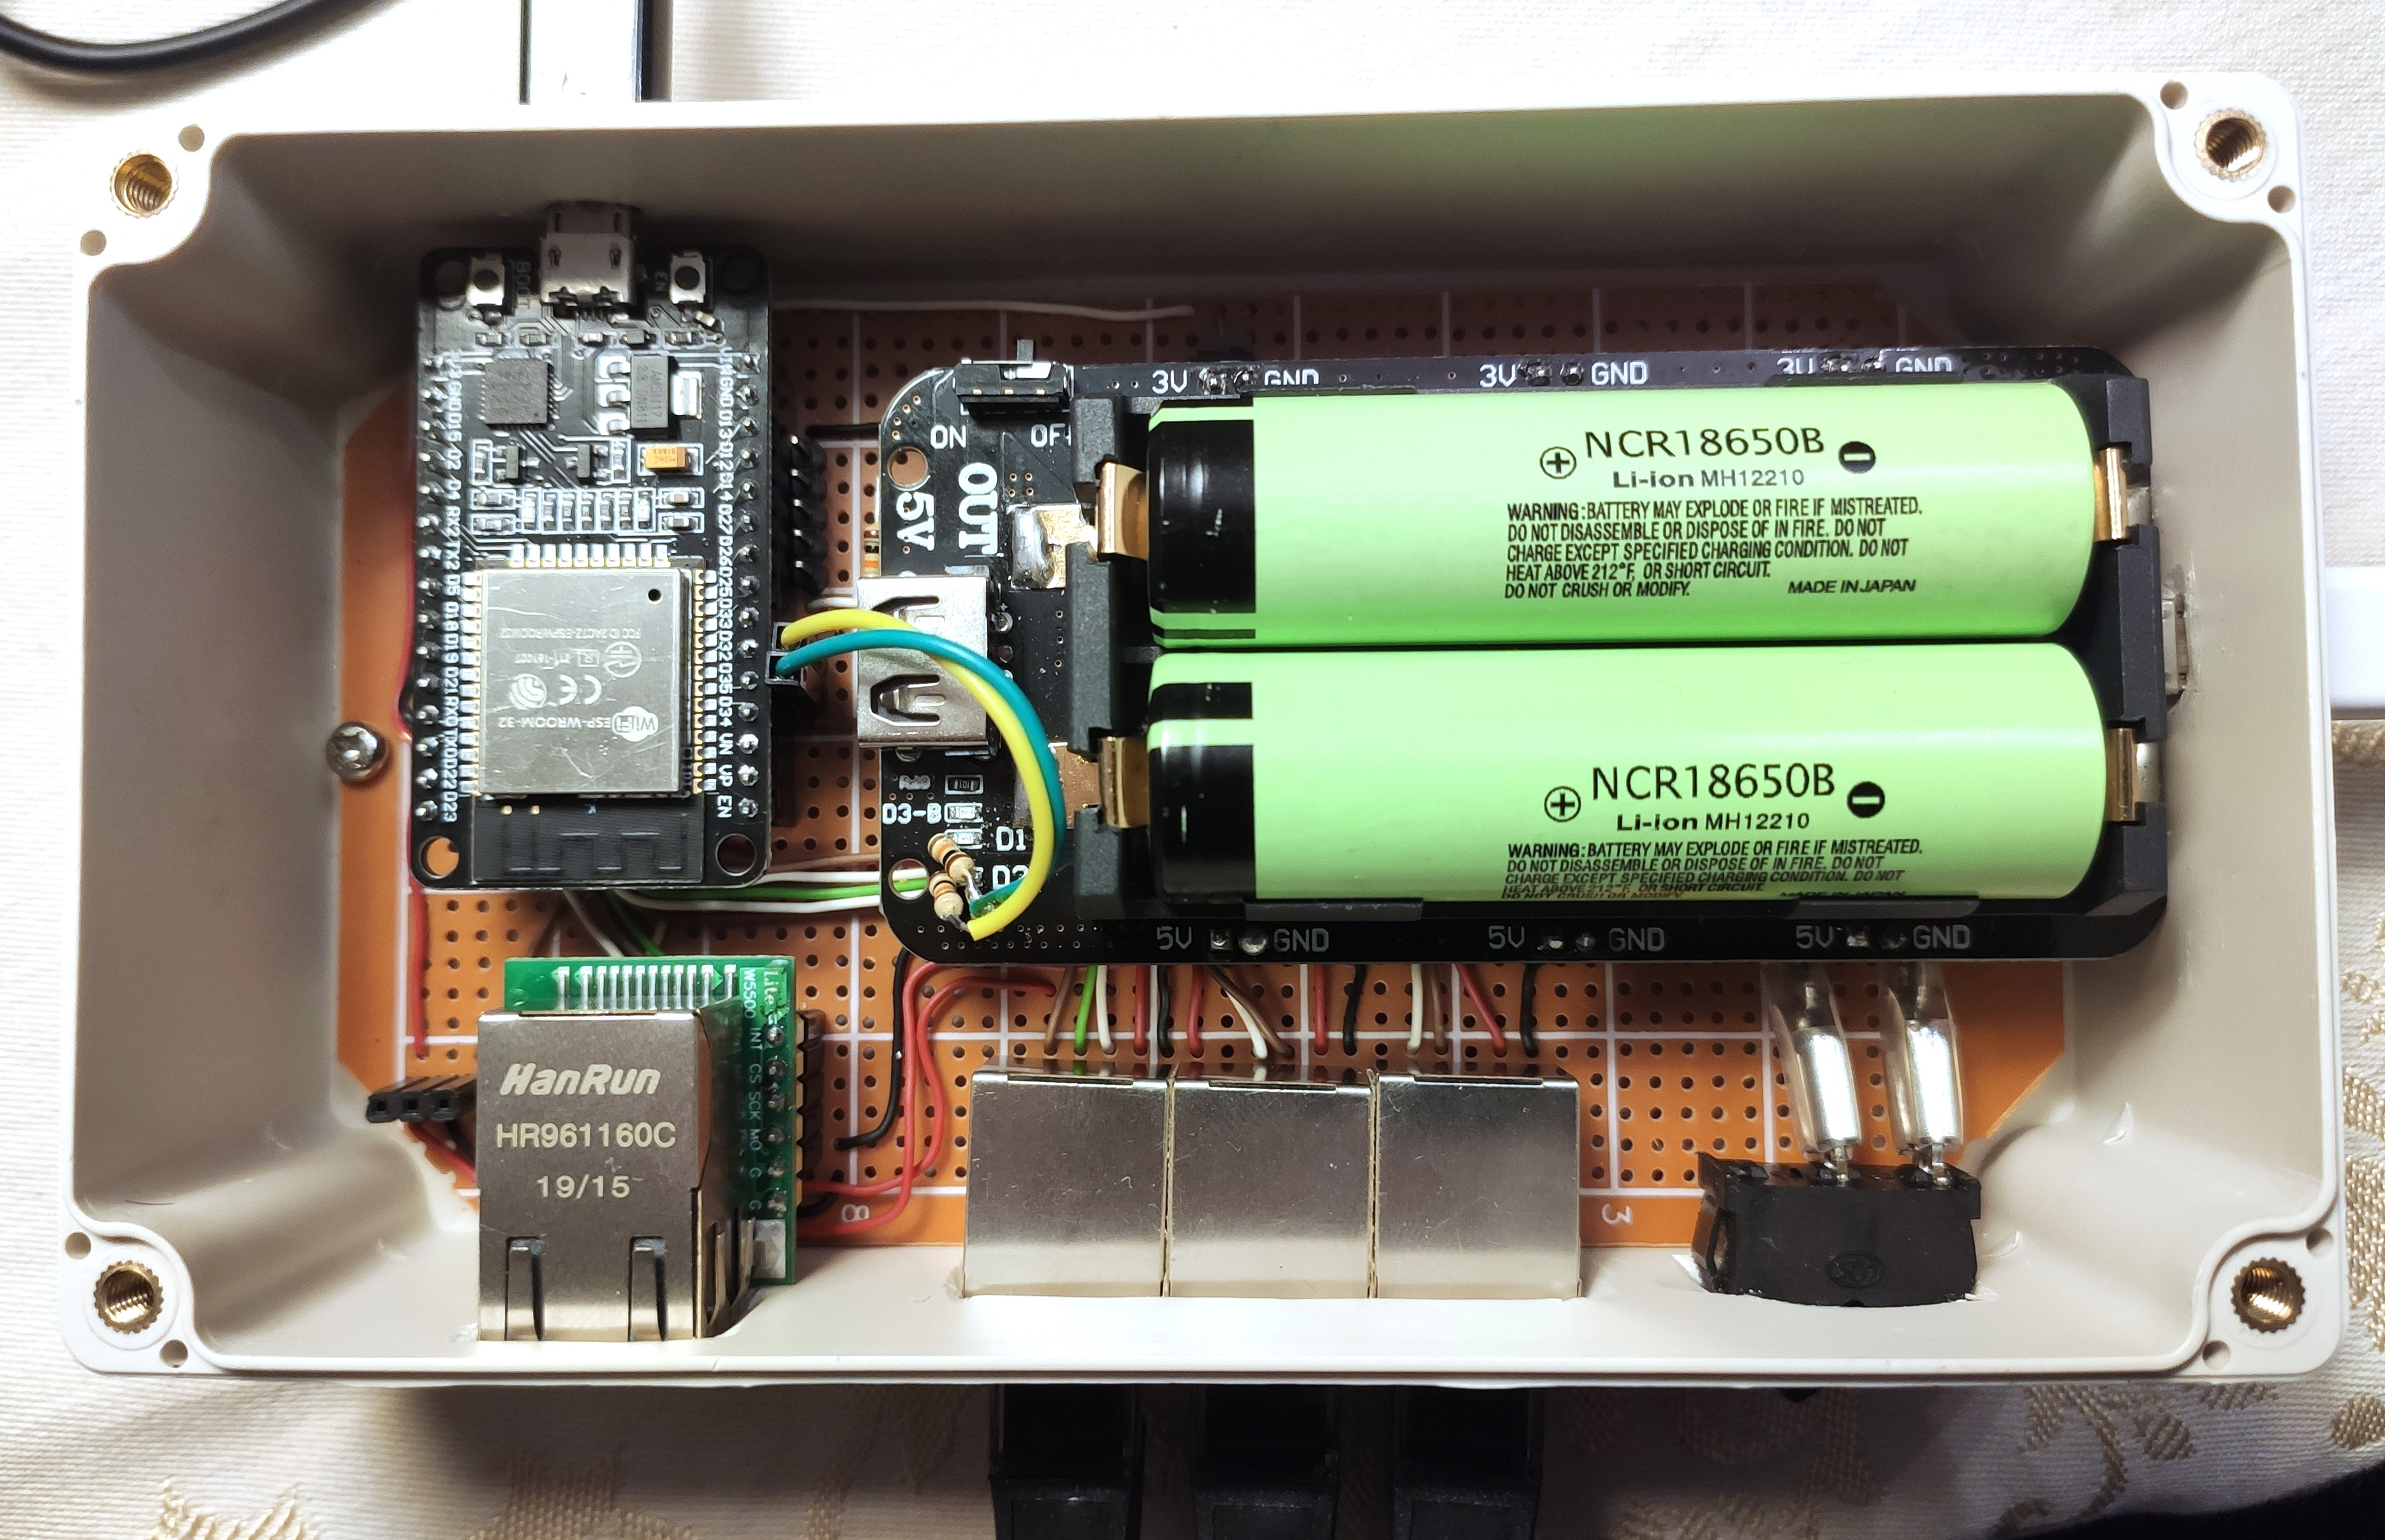
\includegraphics[width=0.8 \textwidth]{fig/wnetrze.jpg}
\caption{Spodnia część obudowy wraz z komponentami sterownika. (opracowanie własne)}
\label{fig:wnetrze}
\end{figure}
 
 \chapter{Opracowanie oprogramowania -~część druga}\label{ch:oprog:2}
  \chaptermark{Opracowanie oprogramowania II}
 W niniejszym rozdziale opisano dalszą część tworzenia oprogramowania sterownika, skupiając się na doskonaleniu i rozbudowie poszczególnych modułów oprogramowania o nowe funkcje i udogodnienia dla potencjalnego użytkownika.

  \section{Rozbudowa portalu przechwytującego}
  W portalu przechwytującym zaprogramowano funkcję, wywoływaną w pętli głównej, podejmującą próbę połączenia z zapamiętaną siecią WiFi w przypadku utraty łączności.
  
 \section{Rozbudowa obsługi termometru i czujnika wilgotności DHT22}
W pliku dht.cpp stworzono funkcję pozwalającą na przekazanie indeksu cieplnego do zmiennej. Postanowiłem wykorzystać go jako punkt odniesienia dla sterownika zamiast temperatury, gdyż precyzyjniej oddaje on warunki termiczne panujące w pomieszczeniu. Dla zabezpieczenia poprawnej pracy sterownika, w przypadku niepowodzenia odczytu lub wątpliwych wartości temperatury i wilgotności (na podstawie których obliczany jest indeks cieplny), funkcja zwraca informację o błędzie.

 \section{Rozbudowa obsługi termopary z modułem MAX6675}
 W celu zabezpieczenia poprawnej pracy sterownika funkcja zwraca wartość 999 stopni Celsjusza oraz wypisuje komunikat o błędzie w przypadku: braku odczytu temperatury, wartości odbiegającej od stanu faktycznego w porównaniu z poprzednimi pomiarami. Zwrócenie przez funkcję tak wysokiej temperatury spowoduje szybkie zamknięcie przepustnicy przez regulator PID, co będzie chroniło piec przed przegrzaniem.
 
 \section{Rozbudowa obsługi wyświetlacza LCD}
 Z obsługi LCD usunięto metodę testową. Dodano funkcję wyświetlającą podstawowe nastawy sterownika: zadaną temperaturę w kominie, aktualną temperaturę w kominie, zadany indeks cieplny w pomieszczeniu, aktualny indeks cieplny w pomieszczeniu oraz procentowe otwarcie przepustnicy. Napisano również funkcję, pozwalająca na włączanie podświetlenia LCD i wyłączanie go po zadanym czasie.

 \section{Rozbudowa obsługi serwomechanizmu}
 Obsługę serwomechanizmu uzupełniono o wyłączanie sygnału sterującego po zmianie pozycji, co w znacznym stopniu przyczyniło się do poprawy kultury pracy. Często występującym problemem było blokowanie się przepustnicy, ze względu na duże opory, przy nieznacznej zmianie wychylenia. Po wyłączeniu sygnału PWM serwomechanizm zaprzestaje prób usytuowania się w zadawanej pozycji i zostaje w tej, którą osiągnął wcześniej. Zapobiega to niepotrzebnemu poborowi energii oraz redukuje głośny dźwięk wydawany przez urządzenie.

 \section{Rozbudowa obsługi regulatora PID}
 W celu poprawy komfortu termicznego w pomieszczeniu, wykorzystano dwa regulatory PID. Pierwszy z nich, na podstawie aktualnej temperatury w pomieszczeniu i zadanej temperatury, oblicza zadaną temperaturę dla spalin w kominie. Drugi, na podstawie aktualnych odczytów temperatury z komina i temperatury zadanej przez pierwszy z regulatorów, oblicza wychylenie serwomechanizmu, a co za tym idzie, stopień otwarcia przepustnicy powietrza dolotowego do komory spalania.
 Dla większej odporności na błędy, dodano funkcje sprawdzające poprawność wartości wejściowych oraz tych obliczanych przez regulatory. Dodatkowo stworzono funkcję wypisującą powyższe wartości na port szeregowy.

 \section{Rozbudowa obsługi termometru Dallas DS18B20}
 Obsługę termometru Dallas uzupełniono o sprawdzanie odczytywanej wartości oraz informowanie o błędnym odczycie.

 \section{Rozbudowa obsługi modułu Ethernet W5500}
 Wbrew wcześniejszym założeniom, nie udało się w przyjętym czasie przenieść komunikacji z radiowej na kablową.
Biblioteka arduino-webthings, przy pracy z mikrokontrolerem ESP32, domyślnie wykorzystuje tylko połączenie WiFi. Aby umożliwić wykorzystanie połączenia Ethernetowego, potrzebne są zwiększone nakłady pracy.
  Obsługa modułu Ethernet W5500 została jedynie poszerzona o funkcje z biblioteki, sprawdzające rodzaj wykrytego urządzenia oraz status połączenia kablowego.
 
 \section{Rozbudowa obsługi odczytu napięć}
 Obsługę odczytu napięć, uzupełniono o funkcję rozpoznającą źródło zasilania, która na podstawie dobranych doświadczalnie wartości progowych, cyklicznie przekazuje wyniki do części programu obsługującej WebThings.
 
 \section{Rozbudowa obsługi wykrywania dotyku}
 Moduł rozpoznawania dotyku uzupełniono o funkcję automatycznie dobierającą wartości progowe, zaraz po uruchomieniu sterownika. Dodano funkcję włączającą wyświetlacz LCD po wykryciu dotyku. Ponadto, utworzono funkcję, wysyłającą cyklicznie odczytywane przez detekcję dotyku wartości do części programu obsługującej WebThings.
 
 \section{Rozbudowa obsługi brzęczyka}
 Do obsługi brzęczyka dodano funkcję włączającą oraz wyłączającą alarm.
 
 \section{Rozbudowa obsługi WebThings}
 Serwer WebThings uzupełniono o 6 różnych urządzeń, dla których określono właściwości zgodne z WoT Capability Schemas \cite{wotschemas2020}:
 \begin{enumerate}
 \item[•] Sensor DHT22 posiada dwie własności: temperaturę (TemperatureProperty) i wilgotność (LevelProperty).
 \item[•] Sensor termopary posiada jedynie własność temperatury (TemperatureProperty).
 \item[•] Sensor PID posiada 6 własności: stopień otwarcia przepustnicy pieca (LevelProperty), temperaturę pomieszczenia (TemperatureProperty), zadaną temperaturę pomieszczenia (TargetTemperatureProperty), własność grzanie/chłodzenie (HeatingCoolingProperty), temperaturę w kominie (TemperatureProperty) oraz zadaną temperaturę w kominie (TemperatureProperty).
 \item[•] Sensor Dallas posiada jedną własność: temperaturę (TemperatureProperty).
 \item[•] Sensor dotyku posiada 5 własności (OnOffSwitch), po jednej dla każdego pola sensora.
 \item[•] Sensor zasilania posiada dwie własności (OnOffSwitch): zasilanie zewnętrzne oraz bateria pełna.
 \end{enumerate}
 Po określeniu właściwości, należało także przypisać każdej z nich odpowiednie atrybuty, takie jak: tytuł, wielokrotność, jednostkę, tryb odczytu.
 Ostatecznie, do każdego z sensorów, dodano funkcję uaktualniającą wartości w serwerze WebThings.
 \subsection{Napotkane problemy}
 Pierwszym ze znalezionych problemów było zwracanie niepełnego opisu rzeczy webowej w formacie JSON przez serwer WebThings. Przyczyna tkwiła w definiowaniu przez bibliotekę webthing-arduino zbyt małego rozmiaru dokumentu JSON. Po zgłoszeniu problemu na stronie projektu, został on naprawiony poprzez umożliwienie użytkownikom wyboru zwiększonego bufora lub definiowania jego rozmiaru.
 
 Drugim z napotkanych problemów było uaktualnianie tylko jednej z własności sensora, po wywołaniu funkcji update, z biblioteki webthing-arduino. Poszukiwanie rozwiązania przyniosło odpowiedź: przyczyną problemu jest błąd w dodatku WebThing do Bramy Mozilli. Tymczasowym rozwiązaniem, pozwalającym na poprawne przekazywanie wartości do bramy, jest wywoływanie funkcji update po zmianie każdej własności z osobna.

 \section{Testowanie sterownika}
 Po opracowaniu kolejnej części oprogramowania, działanie sterownika było testowane z wykorzystaniem monitora portu szeregowego, poprzez odczytanie mierzonych wartości.


 \chapter[Zintegrowanie sterownika pieca kominkowego\\ z Mozilla Gateway]{Zintegrowanie sterownika pieca kominkowego z Mozilla Gateway}\label{ch:gateway}
  \chaptermark{Zintegrowanie z Mozilla Gateway}
 W tym rozdziale opisany został proces integrowania sterownika pieca kominkowego z Bramą Mozilli.
 
 \section{Przygotowanie lokalnej Bramy WebThings}
  Projekt WebThings Gateway by Mozilla oferuje cztery możliwości instalacji: wykorzystanie obrazu dla Raspberry Pi, wykorzystanie obrazu Docker, użycie pakietu na Arch Linux lub samodzielna budowa ze źródła. Wybrano opcję wykorzystania gotowego obrazu dla Raspberry Pi.
  Po jego wgraniu i uruchomieniu urządzenia należy przejść do procesu konfiguracji \cite{gatewaystarted2019}, połączyć się z daną siecią WiFi, natomiast w portalu przechwytującym wskazać połączenie z jakiego będziemy korzystać. Następnie należy wybrać subdomenę oraz utworzyć konto pierwszego użytkownika. Wtedy brama staje się gotowa do działania.

 \section{Dodanie rzeczy webowych do Bramy WebThings}
 Kolejnym etapem integracji było dodanie stworzonych przez sterownik rzeczy webowych do Bramy. Po włączeniu go i połączeniu z tą samą siecią lokalną co Brama, należy wybrać opcję dodawania urządzeń. Brama automatycznie wykrywa rzeczy webowe i proponuje dodanie poszczególnych sensorów. Większość opcji można pozostawić jako domyślne, potwierdzając tylko dodawanie.
 
 \section{Wykorzystywanie interfejsu Bramy WebThings}
 Dzięki zapewnieniu przez Fundację Mozilli zdalnej usługi tunelowania istnieje możliwość zalogowania się do Bramy WebThings poprzez, wybrany na etapie przygotowania, adres subdomeny oraz login i hasło. Po zalogowaniu się widoczne są aktualne parametry pracy sterownika oraz istnieje opcja zmiany temperatury zadanej w pomieszczeniu. W zakładce "Logs", w interfejsie Bramy WebThings, jest możliwość dodawania wykresów czasowych poszczególnych własności sensorów sterownika. Natomiast zakładka "Rules" umożliwia tworzenie reguł, np.: informujących użytkownika o wzroście temperatury poprzez powiadomienia push.
  Zrzut ekranu~\ref{fig:gateway} przedstawia interfejs Bramy WebThings.
\begin{figure}[ht]
\centering
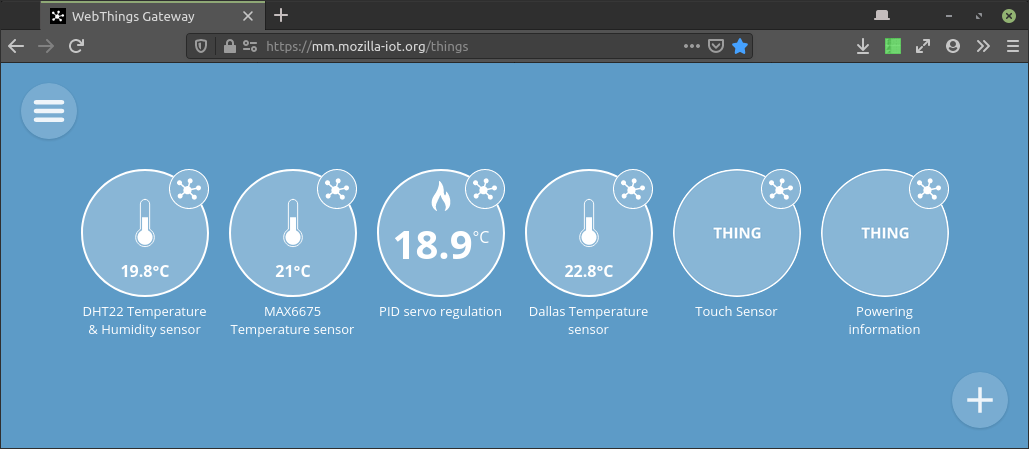
\includegraphics[width=0.8 \textwidth]{fig/gateway.png}
\caption{Interfejs Bramy WebThings. (opracowanie własne)}
\label{fig:gateway}
\end{figure}
 
 \section{Tłumaczenie interfejsu Bramy WebThings}
 Aby poprawić dostępność i wygodę stworzonego rozwiązania, dla osób nie znających języka angielskiego, postanowiono dokonać tłumaczenia interfejsu Bramy WebThings na język polski. Projekt Bramy WebThings umożliwia dodawanie tłumaczeń z wykorzystaniem systemu Fluent \cite{fluent2020}, który zapewnia naturalne brzmienie przekładu. Przygotowane tłumaczenie zostało dodane do projektu Bramy WebThings jako pull request \cite{gatewaypl2019}. Po dokonaniu poprawek, zostało zatwierdzone i będzie dostępne po opublikowaniu najnowszej wersji Bramy WebThings.
 
  \section{Testowanie sterownika}
 Po zintegrowaniu sterownika z Bramą WebThings, przeprowadzono testy manualne z wykorzystaniem interfejsu graficznego Bramy. Ułatwieniem w prowadzeniu testów była możliwość stworzenia wykresów parametrów sterownika w Bramie. 
 
 \chapter{Efekt końcowy na tle koncepcji}
 Z góry narzucony termin wykonania zawsze pozostawia pewien niedosyt, co do zrealizowanego projektu, jednakże wstępny zarys koncepcji został, prawie całkowicie, zrealizowany. To, czego nie udało się osiągnąć, dotyczy
 braku możliwości informowania o zdarzeniach bezpośrednio przez sterownik, za to realizowane jest za pomocą reguły Bramy. Do niepowodzeń można zaliczyć także brak minimalizacji otwarcia przepustnicy w przypadku zaniku napięcia.
 Jednak sterownik spełnia swoje podstawowe zadanie, czyli pozwala na bezobsługową prace paleniska pomiędzy momentami dokładania paliwa, a wykorzystanie serwera WebThings umożliwia korzystanie z Bramy WebThings Mozilli oraz łatwą interakcję sterownika z innymi urządzeniami lub usługami online.
    Zdjęcie~\ref{fig:sterownik} przedstawia kompletny sterownik pieca kominkowego.
\begin{figure}[ht]
\centering
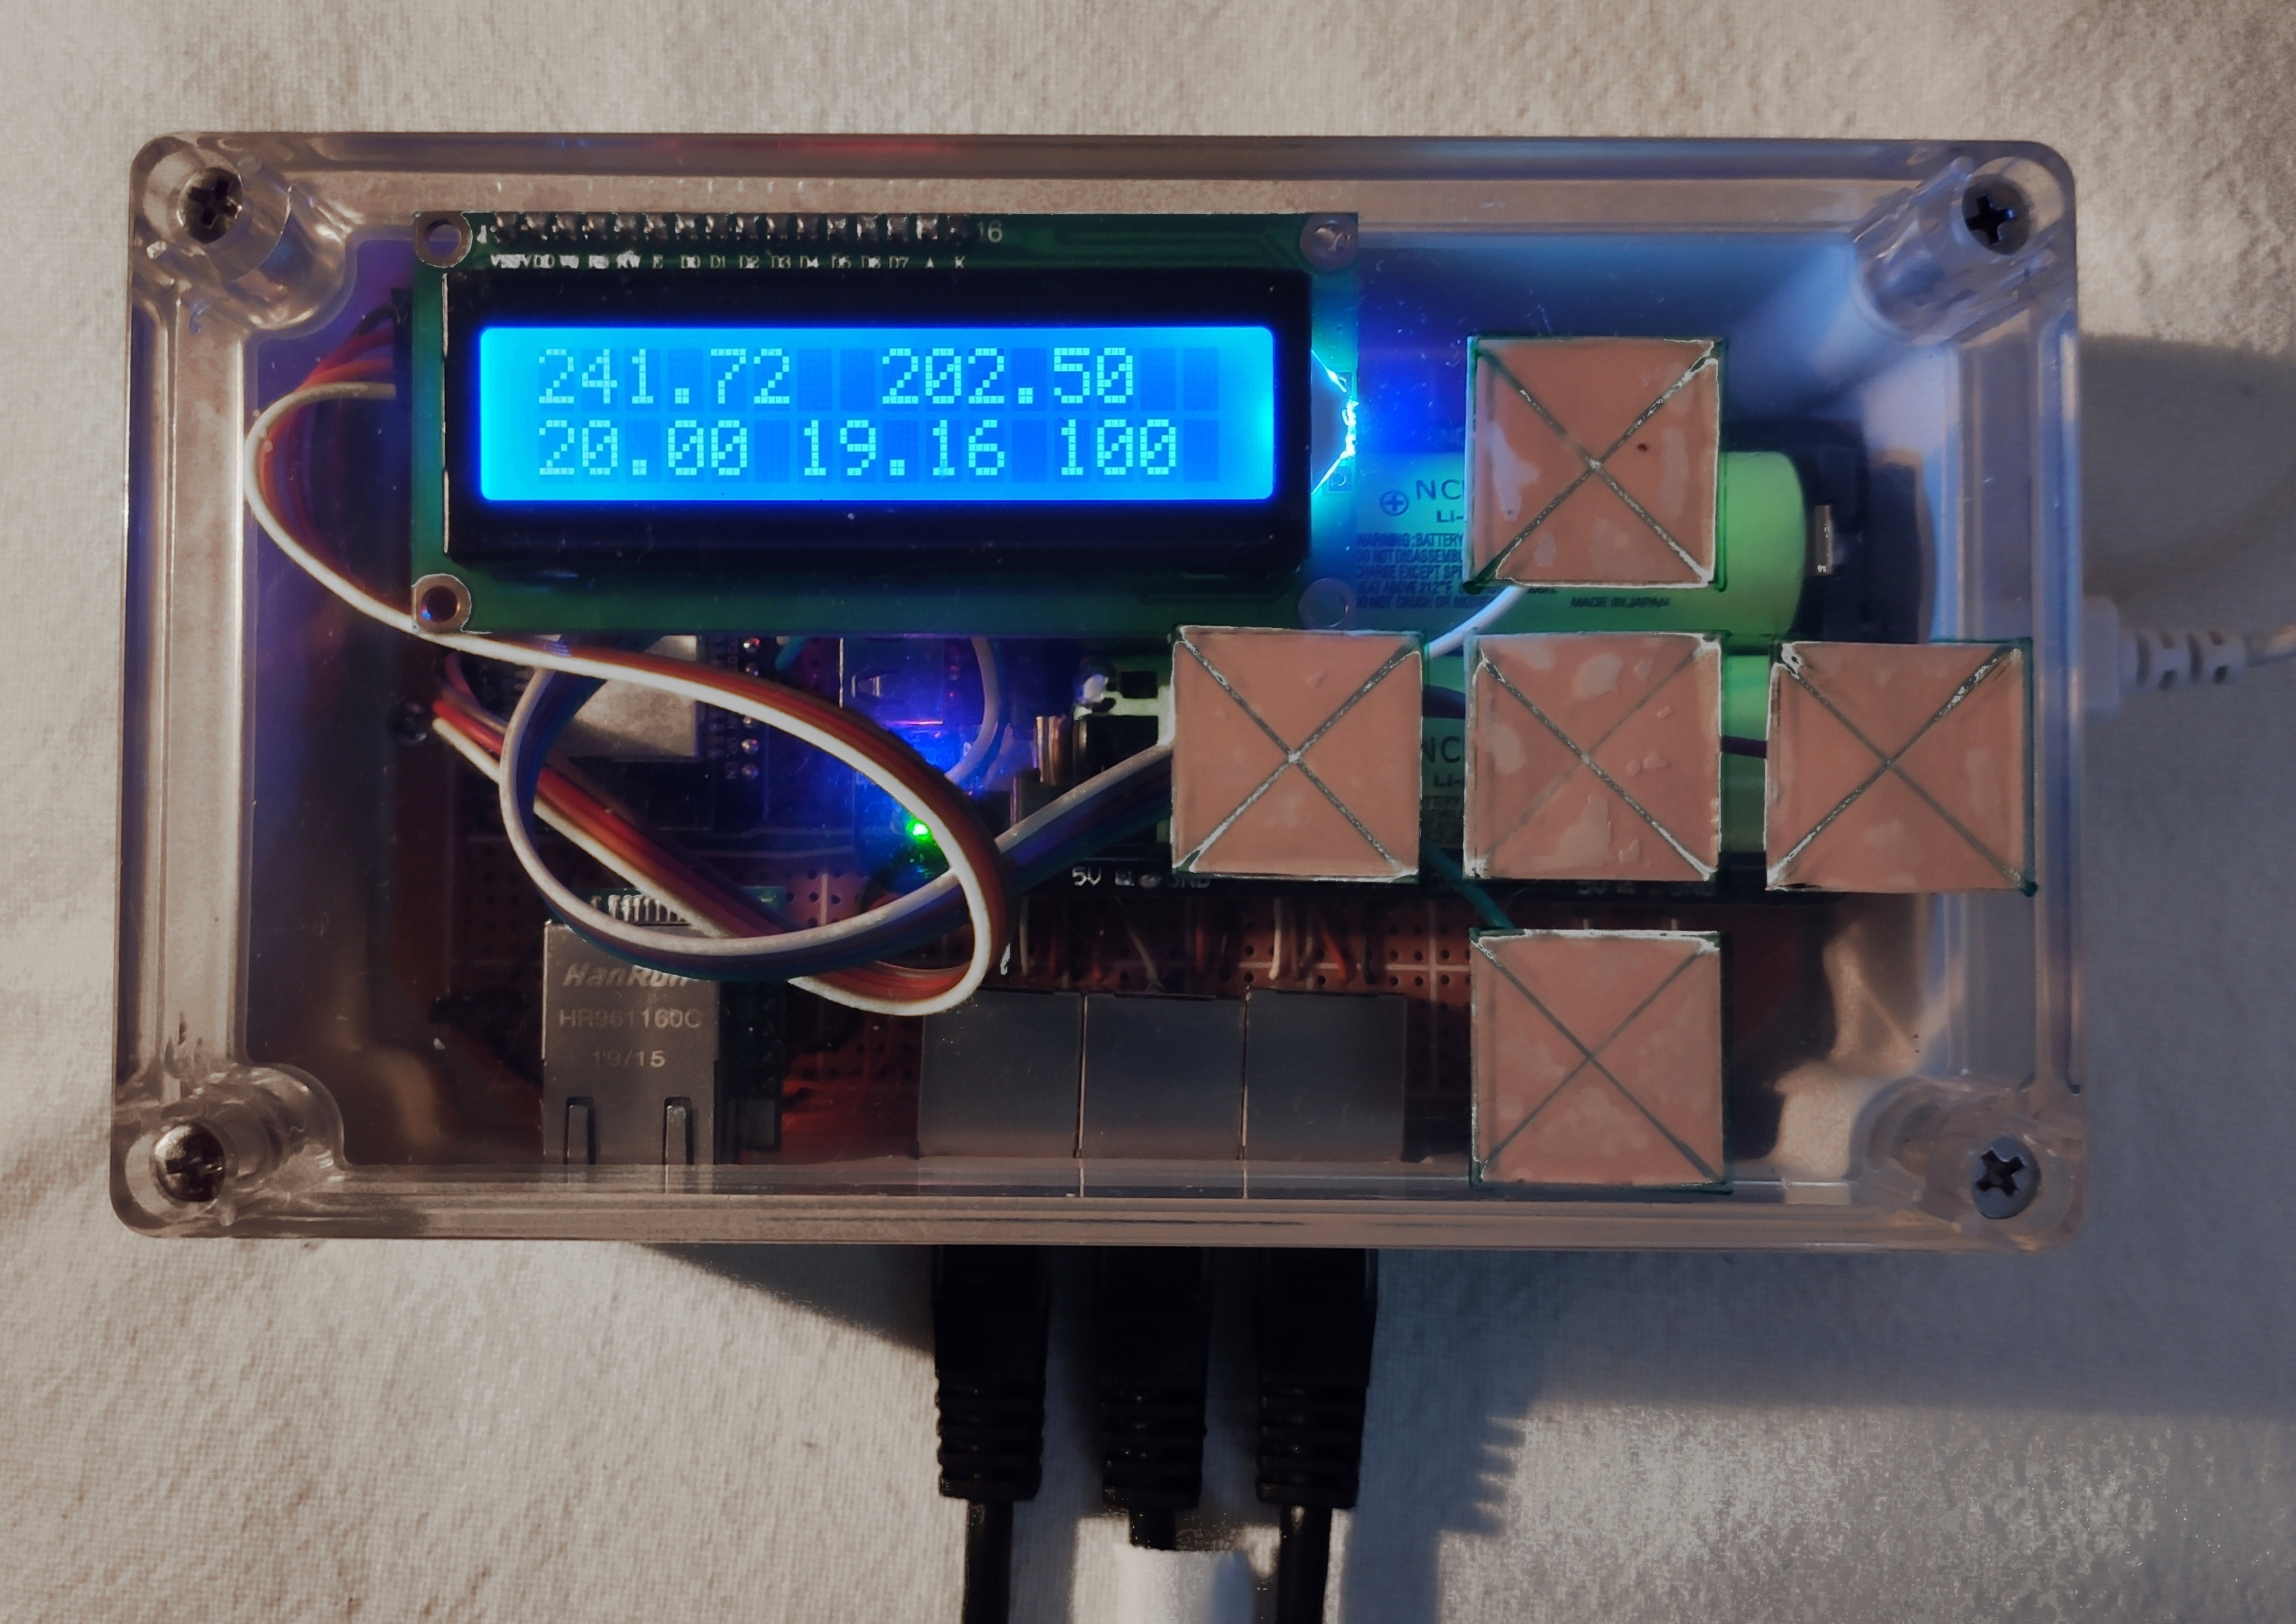
\includegraphics[width=0.8 \textwidth]{fig/sterownik.jpg}
\caption{Kompletny sterownik pieca kominkowego. (opracowanie własne)}
\label{fig:sterownik}
\end{figure}
 
 
 \chapter{Podsumowanie}
W niniejszej części zostaną opisane wnioski z pracy według kolejności wcześniej przedstawionych rozdziałów.

\section{\nameref{ch:przeglad}}
Przegląd istniejącej oferty w tym segmencie pokazał jak mała ilość rozwiązań w zakresie sterowania pieców kominkowych istnieje na polskim rynku, co dowodzi temu, że potrzebne są nowe propozycje produktów.

\section{\nameref{ch:koncepcja}}
Przy tworzeniu koncepcji budowy sterownika pieca kominkowego wyzwaniem było zrozumienie procesu poprawnego spalania drewna. Zadaniem sterownika jest tylko pomoc w utrzymywaniu właściwej temperatury spalin. Ważne jest, aby z jednej strony nie doprowadzić do przegrzania pomieszczenia, a z drugiej nie obniżyć temperatury panującej w piecu na tyle by powodować niedopalanie gazów drzewnych. Niestety, tu główna odpowiedzialność spoczywa na użytkowniku, dlatego ważne jest aby w dołączonej instrukcji obsługi opisać nie tylko samo użytkowanie sterownika, ale i uniwersalne, poprawne zasady palenia w piecu kominkowym.

\section{\nameref{ch:wybor}}
Podczas wybierania podzespołów sterownika pieca kominkowego największą trudność sprawił wybór wśród mnogości dostępnych na rynku rozwiązań. Przeprowadzając analizę wielokryterialną wzięto pod uwagę nie tylko cenę i kompatybilność podzespołów, ale także stopień skomplikowania komunikacji oraz dostępne biblioteki tak, aby nie naruszyć ustalonego terminu oddania projektu.
Głównym wnioskiem jest to, że przy mniejszej docelowej skali wytwarzania końcowych produktów należy wybrać podzespoły droższe, ale o większej skali integracji, na przykład gotową płytkę deweloperską ESP32 z modułem Ethernet. Pomimo, że cena podzespołu jest dwukrotnie wyższa, jego wybór pozwoliłby na znaczną oszczędność czasu poświęconego na łączenie elementów.

\section{\nameref{ch:prototyp:stykowa}}
Wykorzystanie płytki stykowej do tworzenia prototypu nie jest procesem skomplikowanym. Jednak niedostateczna pewność połączeń może sprawiać trudne do wykrycia błędy w komunikacji.
Przy dużej ilości elementów w projekcie należałoby łączyć podzespoły w grupy na osobnych płytkach.

\section{\nameref{ch:oprog:1}}
Największą trudność podczas opracowywania pierwszej - podstawowej - części oprogramowania przyniosło zaznajomienie się z ekosystemem PlatformIO oraz obsługą bibliotek wykorzystanych w projekcie. Aby sprawnie z~nich korzystać należało zapoznać się z licznymi przykładami i wybrać te, które przedstawiają poprawne koncepcje projektowe.

\section{\nameref{ch:prototyp:uniwersalna}}
Wykonanie prototypu na płytce uniwersalnej wymagało dobrych zdolności manualnych, precyzji wykonania oraz umiejętności posługiwania się lutownicą. W ciasnym sąsiedztwie wylutowywanie błędnie umieszczonych elementów sprawiało dużą trudność.
Wybór portów 8p8c, z wyprowadzeniami w rastrze 2,54mm, lub tych, umieszczonych na płytkach drukowanych, znacznie ułatwiłby proces łączenia ich z płytką uniwersalną.
Praca włożona w konstrukcję prototypu na płytce uniwersalnej pozwoliła na niezawodne połączenie komponentów sterownika i dała większą pewność przy opracowywaniu oprogramowania.

\section{\nameref{ch:obudowa}}
Tworzywo plastikowe, wykorzystane do stworzenia skrzynki, umożliwiło łatwe wycięcie otworów na porty komunikacyjne sterownika.

\section{\nameref{ch:oprog:2}}
W drugiej części opracowywania oprogramowania największą trudność sprawiło wykorzystanie biblioteki arduino-webthings, ponieważ jest to nowy zestaw komponentów programu, nie posiadający jeszcze doprecyzowanej dokumentacji. Podczas opracowywania kodu programu, przyczyną znaczącego spowolnienia pracy były błędy znajdujące się nie w kodzie użytkownika, a w bibliotece.
Wykorzystywanie oprogramowania we wczesnym stadium rozwoju zawsze wiąże się z ryzykiem występowania niezidentyfikowanych jeszcze błędów i niekompletną dokumentacją, dlatego potrzebny jest znaczny zapas czasu na rozwiązanie nieprzewidzianych problemów.

\section{\nameref{ch:gateway}}
Uaktualnianie poprzednich wersji Bramy WebThings doprowadziło do jej wadliwego działania.
Podczas testów, stosowanie dużej ilości wykresów, a w konsekwencji zwiększonej liczby zapisów i odczytów z karty pamięci, doprowadziło do jej szybkiej degradacji i konieczności wymiany.
Bardziej efektywnym rozwiązaniem byłoby zastosowanie innej platformy zamiast Raspberry Pi, która nie posiada wbudowanej pamięci, oraz skorzystanie z obrazu Dockera.
 
 \chapter{Dalszy kierunek prac}
Posiadając wiedzę uzyskaną w trakcie tworzenia projektu podszedłbym inaczej do problemu opracowania koncepcji oraz wykonania sterownika pieca kominkowego. Przede wszystkim wykorzystałbym inne źródło zasilania awaryjnego, dające bezpośrednio więcej informacji o stanie baterii. Wykorzystałbym też płytkę deweloperską mikrokontrolera ESP32 z większą ilością wyprowadzeń, tak aby pozostawić sobie pole do rozszerzenia liczby podłączonych czujników. W kwestii programowej, poświęciłbym dodatkowy czas, aby stworzyć testy jednostkowe, których zabrakło w tej wersji oprogramowania.

Podjętym bezpośrednio, dalszym kierunkiem pracy będzie poprawa bezpieczeństwa funkcjonowania sterownika tak, aby piec kominkowy nie wymagał nadzoru na dłuższy czas.
Kolejnym krok stanowić będzie podział pracy pieca kominkowego na odrębne fazy i opracowanie do nich indywidualnych podprogramów. Następnie stworzone zostanie menu użytkownika wyświetlane na LCD.
W dalszej kolejności komunikacja z internetem zostanie przeniesiona z WiFi na połączenie Ethernet.



 \inputencoding{utf8}
 
 \newpage
 \addcontentsline{toc}{chapter}{Książki}
 \printbibliography[title={Książki},type=book]
 
 \addcontentsline{toc}{chapter}{Artykuły}
 \printbibliography[title={Artykuły},type=article]
 
 \addcontentsline{toc}{chapter}{Prace dyplomowe}
 \printbibliography[title={Prace dyplomowe}, type=thesis]
 
 \addcontentsline{toc}{chapter}{Materiały konferencyjne}
 \printbibliography[title={Materiały konferencyjne},type=inproceedings]
 
 \addcontentsline{toc}{chapter}{Pozostałe źródła}
 \printbibliography[title={Pozostałe źródła}, nottype=article, nottype=book, nottype=inproceedings, nottype=thesis]

 \end{document}
